\documentclass[undefended]{sfuthesis}

\title{A Review of the Viscous Burgers' Equation with a focus on Numerical Solutions}
\thesistype{Thesis}
\author{Jarren Ralf}
\previousdegrees{}
\degree{Bachelor of Science (Honours)}
\discipline{Applications of Mathematics}
\department{Department of Mathematics}
\faculty{Faculty of Science and Horticulture}
\copyrightyear{2019}
\semester{Spring 2019}
\date{\today}

\keywords{Burgers' equation; Cole-Hopf transformation; diffusion equation; finite differences; finite elements; numerical solutions}

\committee{\member{Louis Saumier}{Senior Supervisor\\Professor}}

\usepackage[framed, numbered]{matlab-prettifier}
\usepackage{booktabs, tabularx, threeparttable}
\usepackage[linesnumbered, ruled]{algorithm2e}
\usepackage[pdfborder={0 0 0}]{hyperref}
\usepackage{amsmath, amssymb, amsthm}
\usepackage{pgfplots, tikz}
\usepackage{bm, graphicx}

\pgfplotsset{samples = 1000}
\usepgfplotslibrary{fillbetween}

\frenchspacing
\renewcommand*{\chapterautorefname}{Chapter}
\renewcommand*{\sectionautorefname}{Section}
\renewcommand*{\subsectionautorefname}{Section}

\begin{document}

\frontmatter
\maketitle{}
\makecommittee{}

\begin{abstract}
	The viscous Burgers' equation is a nonlinear Partial Differential Equation (PDE) used in the study of fluid dynamics, traffic flow, and shock theory. Applying the Cole-Hopf transformation converts it into the diffusion equation, which means an exact solution can be found under certain conditions. Nonlinear PDEs are often difficult to solve so that makes Burgers' equation a mathematically significant starting point when developing and testing new nonlinear numerical solvers. In this work, analytical solutions will be presented, with a focus on the Fourier series approximation. Multiple numerical approaches will be shared, including finite differences, finite elements, and spectral methods. A Crank-Nicolson scheme will be highlighted, including an implementation and numerical results. In addition, a finite element approach will be mapped out in detail, with results. 
\end{abstract}

\begin{dedication}
	To my mom Brenda, my dad Jan, and my sister Kristen for their overwhelming support.
\end{dedication}

\begin{acknowledgements}
	I would like to thank all of my instructors at Kwantlen Polytecnic University (KPU) over the years. I am grateful for those who have helped me to discover and cultivate my mathematical interests. A special thanks goes out to Louis Saumier for his passionate guidance with this project and many others. 
\end{acknowledgements}

\addtoToC{Table of Contents}%
\tableofcontents%
\clearpage

\addtoToC{List of Tables}%
\listoftables%
\clearpage

\addtoToC{List of Figures}%
\listoffigures%
\clearpage

\addtoToC{List of Algorithms}%
\listofalgorithms
\clearpage

\mainmatter%

\chapter{Introduction}

Significant work has been done studying non-linear Partial Differential Equations (PDEs) in the context of fluid mechanics. One particular equation that has been examined in great depth is the famous Burgers' equation. This work will be a brief review of some literature, sharing both historical context and significance. Furthermore, analytical and numerical solutions, for a range of boundary and initial conditions, will be briefly described. In order to properly introduce the focus of the paper, a theoretical background of fluid mechanics and the Navier-Stokes equations will be presented in Chapter \ref{sec:background}.

Burgers' equation was first written down by a man named Harry Bateman in 1915 \cite{bateman}, in the form 
\begin{subequations}
\label{burgersEqBateman}
\begin{align}
\frac{\partial u}{\partial t} + u \frac{\partial u}{\partial x} = \kappa \frac{\partial^2 u}{\partial x^2}, \quad 0 < x < L, \quad 0 < t < \tau, \label{burgersEq}
\end{align}
\text{with the following initial and boundary conditions}
\begin{align}
u(x, 0) &= \psi(x), \quad 0 < x < L, \label{initialCond}\\
u(0, t) &= \zeta_1(t), \quad u(L, t) = \zeta_2(t), \quad 0 < t < \tau, \label{boundConds}
\end{align}
\end{subequations}
where $u$ is the velocity, $x$ and $t$ are the spacial and time coordinates, and $\kappa$ is the coefficient of dissipation (assumed always to be positive). Notice that $\psi, \zeta_1$, and $\zeta_2$ are arbitrary functions which can be chosen based on the desired conditions. This equation will be elaborated on in Chapter \ref{sec:burgersEq}.

Johannes Martinus Burgers was born and educated in the Netherlands, which included earning his PhD in 1918 under the supervision of Paul Ehrenfest \cite{ehrenfest}. Burgers' dissertation at the time included research on the quantum theory of the atom, motivated by the recent advances on the subject by Niels Bohr. It was many years later in 1948, when Burgers went on to use equation \eqref{burgersEq} to model turbulence \cite{JMBurger}. Due to his significant contribution to the subject of fluid mechanics, the equation now bears his name.

There are several ways to solve Burgers' equation analytically, as we will see in Chapter \ref{sec:analyticalSolution}, but one such approach stands out. Julian David Cole and Eberhard Hopf independently discovered a transformation that linearizes Burgers' equation into the Diffusion equation. It is now called the Cole-Hopf transformation (more on this in Section \ref{sec:coleHopf}.)

\begin{figure}[h!]
	\begin{minipage}{0.16\textwidth}
		\includegraphics[width=\linewidth]{figures/Harry_Bateman.jpg}
	\end{minipage}\hfill
	\begin{minipage}{0.16\textwidth}
		\includegraphics[width=\linewidth]{figures/Johannes_Burgers.jpg}
	\end{minipage}\hfill
	\begin{minipage}{0.16\textwidth}%
		\includegraphics[width=\linewidth]{figures/Paul_Ehrenfest.jpg}
	\end{minipage}
	\begin{minipage}{0.16\textwidth}%
		\includegraphics[width=\linewidth]{figures/Niels_Bohr.jpg}
	\end{minipage}
	\begin{minipage}{0.16\textwidth}%
		\includegraphics[width=\linewidth]{figures/Eberhard_Hopf.jpg}
	\end{minipage}
	\begin{minipage}{0.16\textwidth}%
		\includegraphics[width=\linewidth]{figures/Julian_Cole.jpg}
	\end{minipage}
	\caption{From left to right: Harry Bateman, Johannes Burgers, Paul Ehrenfest, Niels Bohr, Eberhard Hopf, and Julian Cole.}
	\label{fig:people}
\end{figure}

Most PDEs don't have an analytical solution, and hence a numerical approach has become a strong focus of the subject. This will be the core concept in Chapter \ref{sec:numericalSolutions}. Finite difference schemes will be discussed, along with finite elements and spectral methods. 

Chapter \ref{sec:results} will contain the results of the numerical solutions. They will be compared to each other and to the exact solution\footnote{The exact solution will of course be an approximation using a finite Fourier series. The true solution requires infinitely many terms in the sum.}. 

The final Chapter, Chapter \ref{sec:conclusions}, will give a very brief overview and summary of my senior project.

All of the matlab code used in the creation of this project is given in Appendix \ref{sec:code}.

\chapter{Theoretical Background}
\label{sec:background}

Fluid mechanics is the study of moving gases and liquids. The term gas refers to a material that allows for substantial change in density given an arbitrary region of space within the substance. For clarification, this means the distances between molecules of a gas are, on average, orders of magnitude larger than that of a liquid, which therefore makes it easier to distinguish gases from liquids. The process of differentiating liquids from solids however, is a little more refined. The main consideration would be the tangential shear resistance. If an object can be subjected to this type of force and still maintain one piece, then it would be classified as a liquid; in contrast a solid would break into two or more pieces. 

The second word in the classification of this area of study is mechanics, which in general refers to the study of movement. Motion of this type would be under the designation of Newtonian mechanics. This is because the classical laws of physics derived largely in part by Sir Isaac Newton, are the governing factors of fluids. There are several properties that are important when describing the movement of fluids. The most relevant for this literature review are viscosity, turbulence, and compressibility.

Viscosity describes the internal friction of a fluid. It manifests as a resistance to movement down an incline. If you analyze a slice of fluid (call it a layer) and observe the effects of layers with varying velocities moving past each other, the fast layer will try to curtail the speed of the slower layer with friction. This is a depiction of viscosity. This effect is described in equations using a dimensionless quantity called the Reynolds number, usually denoted $Re$. When the Reynolds number of a substance is low, the fluid would display signs of being highly viscous, observable as smooth laminar-type motion. 

In contrast, high Reynolds numbers are reserved for turbulent phenomena when there is a lot of chaotic movement in the substance. Thus, turbulence is observed in gases and fast flowing liquids. This behavior spawns from tumultuous change in pressure. Observe in Figure \ref{fig:LaminarAndTurbulent} part (b) below, that the turbulent flow has layers of fluid flows that intersect with one another, which is an example of the chaotic behavior that is tough to model.
\begin{figure}[h!]
	\centering
	\includegraphics[width=10cm]{figures/Laminar_and_turbulent.png}
	\caption{Top: Laminar Flow; Bottom: Turbulent Flow}
	\label{fig:LaminarAndTurbulent}
\end{figure}

The effect of pressure to change the size, or region of a substance, is called compressibility. This can be directly described by a change in density, as we will see in the following derivation. An example of compressible fluid would be gases because the particles in a gas have the freedom to move around without being constrained to one another. An incompressible fluid on the other hand is something that keeps its density constant, which includes most liquids. In terms of calculus, compressibility can be described by a quantity called the divergence.

\section{The Navier-Stokes Equations}
\label{sec:navierStokesEq}

This section will begin with a \textit{brief} derivation of the Navier-Stokes equations by means of summarizing the work done by Alexandre Joel Chorin and Jerrold E. Marsden in \textit{A Mathematical Introduction to Fluid Mechanics} \cite{mathematicalIntroFluids}. 

The Navier-Stokes equations are derived from three fundamental principles of physics, namely the conservation of mass, balance of momentum (Newton's second law), and conservation of energy.

\subsection{Conservation of Mass}

Consider some region in space, we will call it $D \in \mathbb{R}^3$ and suppose $\textbf{x}$ is some point in $D$. The velocity of a particle through position $\textbf{x}$ at time $t$ will be denoted by $\textbf{u}(\textbf{x}, t)$. Allow $\rho(\textbf{x}, t)$ to denote the mass density of the fluid. If $W$ is any subregion of $D$, then the mass of fluid in $W$ can be expressed as
\begin{align}
m(W, t) = \int_W \rho (\textbf{x}, t) \,\mathrm{d}V \label{mass}
\end{align}
for some time $t$.

The rate of change of mass in $W$ \eqref{mass}, given that we fix the subregion $W$ in space, is \[\frac{\mathrm{d}}{\mathrm{d} t} m (W, t) = \frac{\mathrm{d}}{\mathrm{d} t} \int_W \rho(\textbf{x}, t) \,\mathrm{d} V = \int_W \frac{\partial \rho}{\partial t}(\textbf{x}, t) \,\mathrm{d} V.\]

We will use the notation $\partial W$ to describe the boundary of the region $W$. Suppose that $\textbf{n}$ denotes the unit outward normal vector, then the mass flow rate per unit area is $\rho \textbf{u} \cdot \textbf{n}$ (see Figure \ref{fig:boundary}). 
\begin{figure}[h!]
\centering
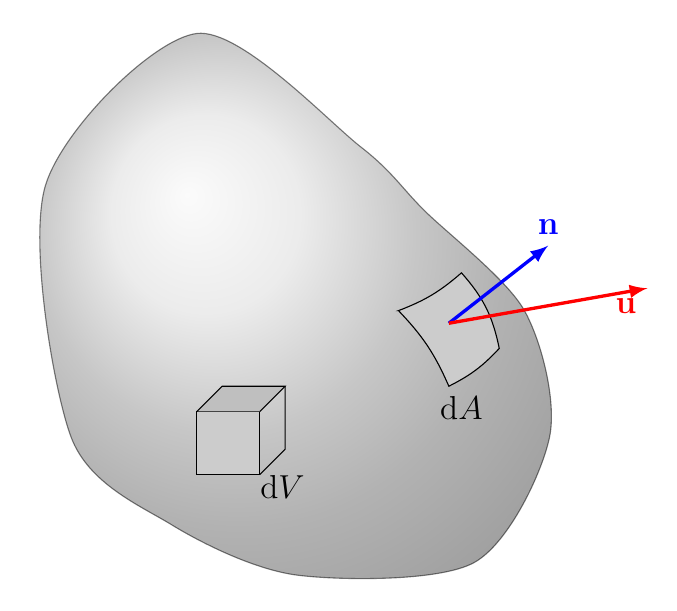
\begin{tikzpicture}[scale=1.6, font=\large]
\shadedraw[ball color=gray!40,opacity=0.5] plot[smooth cycle] coordinates {(-2,1) (-0.8,2.2) (0.5,1.3) (1,0.8) (1.8,0)
	(2,-1) (1.4,-2) (0,-2.1) (-1,-1.7) (-1.8,-1)};
\draw[fill=gray!40] (0.8,0) to[bend right=10] (1.3,0.3) to[bend left=15] (1.6,-0.3)
to[bend left=10] (1.2,-0.6) to[bend right=10] cycle;
\draw[blue,very thick,-latex] (1.2,-0.1) -- ++(38:1) node[above] {$\textbf{n}$};
\draw[red,very thick,-latex] (1.2,-0.1) -- ++(10:1.6) node[below left] {$\textbf{u}$};
\node[anchor=north] at (1.3,-0.6) {d$A$}; 
\draw[fill=gray!40] (-0.8,-0.8) rectangle (-0.3,-1.3) node[below right=0pt,
inner sep=0pt]{d$V$};
\draw[fill=gray!50] (-0.8,-0.8) -- ++ (0.2,0.2) -- ++ (0.5,0) -- (-0.3,-0.8);
\draw (-0.3,-1.3) -- ++ (0.2,0.2) -- ++ (0,0.5);
\end{tikzpicture}
\caption{The normal vector with respect to the surface $W$ relates to the flow rate of the mass crossing the boundary, $\partial W$, by $\rho \textbf{u} \cdot \textbf{n}$ per unit area.}
\label{fig:boundary}
\end{figure}

This leads to the integral form of the law of conservation of mass, 
\begin{align}
\frac{\mathrm{d}}{\mathrm{d} t} \int_W \rho \,\mathrm{d}V = - \int_{\partial W} \rho \textbf{u} \cdot \textbf{n} \,\mathrm{d} A. \label{lawConservationMass}
\end{align}
Recall that the divergence of $\textbf{u}$ describes the flux in a small region of space. Given this, we can see that equation \eqref{lawConservationMass} is equivalent to \[\int_W \left[\frac{\partial \rho}{\partial t} + \mathrm{div}(\rho \textbf{u})\right] \,\mathrm{d} V = 0\] by the divergence theorem. Again this is also equivalent to 
\begin{align}
\frac{\partial \rho}{\partial t} + \mathrm{div}(\rho \textbf{u}) = 0 \label{conservationMassEq}
\end{align}
because it holds for all $W$. This is one of the forms that conservation of mass is expressed as, called the differential form.

\subsection{Balance of Momentum}

To formulate Newton's second law, we must first be able to describe the path of a particle in space. Naturally we start with the position as a function of time, denoted $\textbf{x}(t) = (x(t), y(t), z(t)).$ Obviously velocity is a time derivative of this quantity, as shown below \[\textbf{u}(x(t), y(t), z(t), t) = (\dot{x}(t), \dot{y}(t), \dot{z}(t)) = \textbf{u}(\textbf{x}(t), t).\]

Taking one more time derivative leads us to the acceleration of the particle, displayed in the form below \[\textbf{a}(t) = \frac{\mathrm{d}}{\mathrm{d} t} \textbf{u} (x(t), y(t), z(t), t) = \frac{\mathrm{d}}{\mathrm{d} t} \textbf{u}(\textbf{x}(t), t).\] Notice the above equation requires us to use the chain rule from calculus, so now the acceleration becomes \[\textbf{a}(t) = \frac{\partial \textbf{u}}{\partial x} \dot{x} + \frac{\partial \textbf{u}}{\partial y} \dot{y} + \frac{\partial \textbf{u}}{\partial z} \dot{z} + \frac{\partial \textbf{u}}{\partial t}.\]
Introducing a re-parameterization on $\textbf{u}$ the following can be defined \[\textbf{u}(x, y, z, t) = (u(x, y, z, t), v(x, y, z, t), w(x, y, z, t)).\] Now reformulating the derivatives using Euler's notation, as well as the equation above, leads us to \[a(t) = u \textbf{u}_x + v \textbf{u}_y + w \textbf{u}_z +  \textbf{u}_t.\] Finally, the acceleration can be written in a more compact way using the gradient operator, $\nabla$, as shown below \[\textbf{a}(t) = \partial_t \textbf{u} + \textbf{u} \cdot \nabla \textbf{u}\] where \[\partial_t \textbf{u} = \frac{\partial \textbf{u}}{\partial t}, \quad \text{ and } \quad \textbf{u} \cdot \nabla = u \frac{\partial}{\partial x} + v \frac{\partial}{\partial y} + w \frac{\partial}{\partial z}.\]

The material derivative is an operator defined by
\begin{align}
\frac{D}{Dt} = \partial_t + \textbf{u} \cdot \nabla. \label{materialDeriv}
\end{align}
To put it in basic terms, this operator is a way to describe the temporal rate of change with respect to some quantity of a particular fluid parcel moving with the fluid.   

We now have a description of the acceleration, the next step is to derive an expression for the force. The first step in this process is to introduce pressure, $p(\textbf{x}, t)$. Now imagine some smooth surface in our fluid, which we will call $S$. The force across $S$ per unit area will be in terms of the pressure and unit normal, $p(\textbf{x}, t) \textbf{n}$ (see Figure \ref{fig:pressure}).
\begin{figure}[h!]
\centering
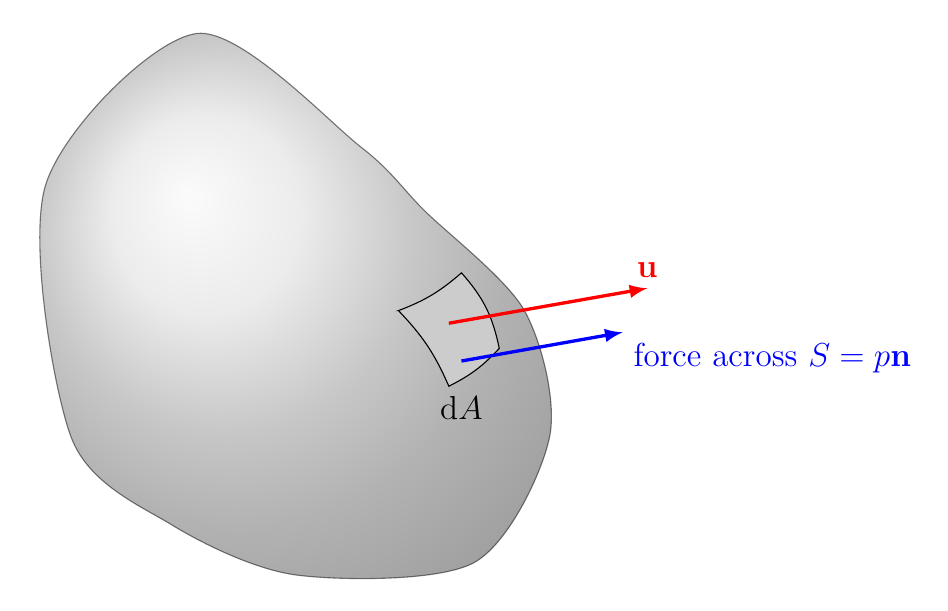
\begin{tikzpicture}[scale=1.6, font=\large]
\shadedraw[ball color=gray!40,opacity=0.5] plot[smooth cycle] coordinates {(-2,1) (-0.8,2.2) (0.5,1.3) (1,0.8) (1.8,0)
	(2,-1) (1.4,-2) (0,-2.1) (-1,-1.7) (-1.8,-1)};
\draw[fill=gray!40] (0.8,0) to[bend right=10] (1.3,0.3) to[bend left=15] (1.6,-0.3)
to[bend left=10] (1.2,-0.6) to[bend right=10] cycle;
\draw[red,very thick,-latex] (1.2,-0.1) -- ++(10:1.6) node[above] {$\textbf{u}$};
\draw[blue,very thick,-latex] (1.3,-0.4) -- ++(10.1:1.3) node[below right] {force across $S = p\textbf{n}$};
\node[anchor=north] at (1.3,-0.6) {d$A$}; 
\end{tikzpicture}
\caption{Pressure forces across a surface $S$.}
\label{fig:pressure}
\end{figure}

Now imagine the pressure as a way of exerting a force on the boundary of the surface $S$, the notation for this will be $\textbf{S}_{\partial W}.$ In integral form, the total force exerted on the surface would be \[\textbf{S}_{\partial W} = - \int_{\partial W} p \textbf{n} \,\mathrm{d} A,\] where the sign is negative because the direction is opposite compared to the outward facing normal. Next we apply the divergence theorem, but first we must consider any fixed vector in space, say $\textbf{e}$, then we can express the force and the dot product of vector $\textbf{e}$ as the following \[\textbf{e} \cdot \textbf{S}_{\partial W} = - \int_{\partial W} p \textbf{e} \cdot \textbf{n} \,\mathrm{d} A = - \int_W \mathrm{div}(p \textbf{e}) \,\mathrm{d} V = - \int_W (\mathrm{grad} \,p) \cdot \textbf{e} \,\mathrm{d} V\] where $\mathrm{grad}$ is the gradient operator, similarly denoted $\nabla$. This implies that \[\textbf{S}_{\partial W} = - \int_W \mathrm{grad} \,p \,\mathrm{d} V.\]

Allow $\textbf{b}(\textbf{x}, t)$ to denote the given body force per unit mass. The total body force is \[\textbf{B} = \int_W \rho \textbf{b} \,\mathrm{d}V.\] We now have that \[\text{force per unit volume} = - \mathrm{grad} \,p + \rho \textbf{b}\] on any piece of material, therefore by Newton's second law we arrive at \[\rho \frac{D \textbf{u}}{Dt} = - \mathrm{grad} \,p + \rho \textbf{b},\] the differential form of balance of momentum. It can be shown that this is equivalent to the following expression,
\begin{align}
\frac{\mathrm{d}}{\mathrm{d} t} \int_{W_t} \rho \textbf{U} \,\mathrm{d} V = S_{\partial W_t} + \int_{W_t} \rho \textbf{b} \,\mathrm{d} V,\label{balanceMomentumEq} 
\end{align}
which is the law of balance of momentum in it's integral form.

\subsection{Conservation of Energy}
\label{sec:ConservationOfEnergy}

Since we are about to evoke the conservation of energy now, we start with the kinetic energy for fluid moving within a subregion $W$, \[E_{\mathrm{kinetic}} = \frac{1}{2} \int_W \rho \|\textbf{U}\|^2 \,\mathrm{d} V,\] where $\|\textbf{U}\|^2 = (u^2 + v^2 + w^2)$ is the squared length of the vector $\textbf{u}.$ Next, we are required to consider what the total energy of the system must be \[E_{\mathrm{total}} = E_{\mathrm{kinetic}} + E_{\mathrm{internal}}.\] The internal energy is an acknowledgement of the internal molecular vibrations that exist. Whereas the kinetic energy is due to the motion of the fluid itself.

The following result follows from computing the rate of change of kinetic energy \[ \frac{\mathrm{d}}{\mathrm{d} t} E_{kinetic} = \int_{W_t} \rho \left(\textbf{u} \cdot \left(\frac{\partial \textbf{u}}{\partial t} + (\textbf{u} \cdot \nabla) \textbf{u} \right)\right). \] From physics we also know that the rate of change of energy must be the same as the rate of which work is done. This leads to the result \[\frac{\mathrm{d}}{\mathrm{d} t} E_{total} = \frac{\mathrm{d}}{\mathrm{d} t} \int_{W_t} \rho \textbf{u} \cdot \textbf{b} \,\mathrm{d} V - \int_{\partial W_t} p \textbf{u} \cdot \textbf{n} \,\mathrm{d} A.\] From this, Euler's equations for isentropic flow, which is flow through a narrow opening without increase or decrease in entropy, can be written down
\begin{align*}
\frac{\partial \textbf{u}}{\partial t} + (\textbf{u} \cdot \nabla)\textbf{u} &= - \nabla w + \textbf{b}, \\
\frac{\partial \rho}{\partial t} + \mathrm{div} (\rho \textbf{u}) &= 0
\end{align*}
in $D$, and where $w$ is the enthalpy per unit mass, which is related to the first law of thermodynamics. Enthalpy is a measure of the total heat content in a system.

At this stage, the force on a supposed surface $S$ per unit area needs to be formulated as the expression \[ - p(\textbf{x, t}) \textbf{n} + \bm{\sigma} (\textbf{x}, t) \cdot \textbf{n},\] where $\bm{\sigma}$ is a matrix called the stress tensor. Newton's second law brings us to \[\frac{\mathrm{d}}{\mathrm{d} t} \int_{W_t} \rho \textbf{u} \,\mathrm{d} V = - \int_{\partial W_t} (p \cdot \textbf{n} - \bm{\sigma} \cdot \textbf{n}) \,\mathrm{d} A.\] Without giving the derivation, two constants will be presented. Based on the system $\bm{\sigma}$, we get the following equation \[\delta_i = \lambda (d_1 + d_2 + d_3) + 2 \mu d_i, \quad i = 1, 2, 3,\] where $\delta_i$ are the eigenvalues of $\bm{\sigma}$, and $d_i$ are the eigenvalues of the symmetric part of $\nabla \textbf{u}$. Notice this now gives us a relationship between the constants $\lambda$ and $\mu.$ These scalars represent two different coefficients of viscosity. These quantities are related to the Reynolds number introduced in Section \ref{sec:background}. They are a way of describing the internal friction in the fluid.

In preparation for the final aspect of this derivation, the transport theorem will be presented. For any function $f$ of $\textbf{x}$ and $t$,
\begin{subequations}
	\label{transportTheorem}
	\begin{align}
	\frac{\mathrm{d}}{\mathrm{d} t} \int_{W_t} \rho f \,\mathrm{d} V = \int_{W_t} \rho \frac{D f}{D t} \,\mathrm{d} V
	\end{align}
	\text{or}
	\begin{align}
	\frac{\mathrm{d}}{\mathrm{d} t} \int_{W_t}  f \,\mathrm{d} V = \int_{W_t} \left(\frac{\partial f}{\partial t} + \mathrm{div} (f \textbf{u})\right) \,\mathrm{d} V.
	\end{align}
\end{subequations}

From \eqref{conservationMassEq}, \eqref{balanceMomentumEq}, and \eqref{transportTheorem}, and the divergence theorem, we arrive at the Navier-Stokes equations,
\begin{align}
\rho \frac{D\textbf{u}}{Dt} = - \nabla p + (\lambda + \mu) \nabla (\textrm{div} \,\textbf{u}) + \mu \nabla^2 \textbf{u}, \label{navierStokesEq}
\end{align}
where \[\nabla^2 \textbf{u} = \left( \frac{\partial^2}{\partial x^2} + \frac{\partial^2}{\partial y^2} + \frac{\partial^2}{\partial z^2} \right) \textbf{u}\] is the Laplacian of $\textbf{u}$.

\chapter{Burgers' Equation}
\label{sec:burgersEq}

Observing the system of equations \eqref{navierStokesEq}, given at the end of Section \ref{sec:ConservationOfEnergy}, we make the simplifying assumption that our fluids will not have changing material density. Picture a spherical neighbourhood around a molecule such that other molecules do not ever cross the boundary of this neighbourhood. If this condition holds for all small regions within a fluid, then that fluid is incompressible. Therefore the divergence is zero. In addition, assuming that pressure is negligible our system simplifies to the following \[\rho \frac{D\textbf{u}}{Dt} = \mu \nabla^2 \textbf{u}.\] Now we divide both sides by density and make the substitution that $\kappa = \frac{\mu}{\rho}$ leaving us with \[\frac{D\textbf{u}}{Dt} = \kappa \nabla^2 \textbf{u}.\] Recall that $\frac{D}{D t}$ denotes the material derivative operator \eqref{materialDeriv} defined previously. Substituting it in brings us to \[(\partial_t + \textbf{u} \cdot \nabla) \textbf{u} = \kappa \nabla^2 \textbf{u}.\] Before moving forward, we will consider only one spatial dimension. The implication of this is not only that the vector-valued function $\textbf{u}$ becomes a real-valued function $u$, but the gradient and Laplacian become the first and second derivative respectively. Finally we arrived at the viscous Burgers' equation \[\frac{\partial u}{\partial t} + u \frac{\partial u}{\partial x} = \kappa \frac{\partial^2 u}{\partial x^2}\] or expressed with different notation
\begin{align}
u_t + u u_x = \kappa u_{xx}, \label{viscousBurgersEq}
\end{align}
where $\kappa$ is the dissipation constant and can be rewritten in terms as the Reynolds number like so \[\kappa = \frac{1}{Re}.\] The Reynolds number is defined in \cite{mathematicalIntroFluids} by \[Re = \frac{\mathcal{L} \,\mathcal{U}}{\nu}\] where $\mathcal{L}$ is a characteristic length, $\mathcal{U}$ is a characteristic velocity, $\nu$ is the coefficient of kinetic viscosity defined by $\mu/\rho_0$, and $\rho_0$ is a constant density for an incompressible flow (recall from Section \ref{sec:ConservationOfEnergy} where $\mu$ is defined as a coefficient of viscosity). As specified in \cite{mathematicalIntroFluids} the quantities $\mathcal{L}$ and $\mathcal{U}$ are ``chosen in a somewhat arbitrary way.'' Chorin and Marsden derive a dimensionless version of the Navier-Stokes equation where the definition of the Reynolds number arises.

To clarify, in this paper whenever we refer to the viscous Burgers' equation or Burgers' equation, we are talking about \eqref{viscousBurgersEq}.

\section{Physical Significance}
\label{sec:burgersEqPhysicalSignificance}

This section is inspired in part by the great work by Bronkile \textit{et al} \cite{burger1} in their research paper titled ``A systematic literature review of Burgers' equation with recent advances.'' As suggested in their paper, the articles written on Burgers' equation seem to lack historical significance. Bronkile \textit{et al} present many different areas that Burgers' equation has been used. Some of those examples will be presented below.

Burgers' equation is used often as a simplification of the Navier-Stokes equations where it is sometimes referred to as a \textit{toy model} \cite{burger2}. A toy model is a concept that is perhaps better formulated than is implied. It is a model that deliberately makes simplifications, often ignoring aspects of a problem, in order to observe certain characteristics. As seen in the derivation above, Burgers' equation completely lacks the ability to model pressure.

The first and most practical reason for the significance of Burgers' equation is because it is a nonlinear PDE with a well known analytical solution in certain cases. There are several numerical solvers for linear systems of PDEs, but nonlinearity still poses problems. In order to develop a nonlinear numerical solver for PDEs, the designer must be able to check that their technique works. In other words, the error needs to be quantifiable. The easiest way to do this is to compare your approximation to the true solution. In the case of Burgers' equation this becomes possible and is still to this day used for testing nonlinear solvers.

In many cases, in order to model real life situations more accurately, complicated initial conditions need to be invoked. In their unpublished work, Barth and Sukys \cite{nasa} compute exact solutions to Burgers equation with initial conditions that contain discrete random variables. This research is an essential part of the development of numerical schemes to stochastic PDEs with random initial conditions, of which Barth and Sukys are currently formulating.

\subsection{Fluid Dynamics}

Historically the equation has been used in the formulation of viscous and turbulent flows. Work on Burgers' equation started with Bateman \cite{bateman} in 1915, where he proposed equation \eqref{burgersEq} as a way to deal with small values of viscosity. The problem was that the motion of fluid becomes discontinuous as viscosity approaches zero. There is the presence of randomness while dealing with turbulence, so Bec and Kahanin \cite{stochasticBurgers} proposed the use of a multidimensional stochastic Burgers' equation to describe the phenomenon. Probability distribution of velocity gradients were studied by Weinan \textit{et al} \cite{fluidDynamics3}, and in particular the asymptotic behaviour. 

\subsection{Shock Theory}

One of the most well known areas of study that Burgers' equation is often associated with is shock theory. As the viscosity of a fluid decreases and tends to zero, the velocity of the solution starts to become discontinuous (see Figure \ref{fig:shockTheory}). Kreiss and Kreiss \cite{shockTheory} studied the effects of shocks from the viscous Burgers' equation in 1985. They proved that all of the eigenvalues were negative, which helped lead to the uniqueness and existence of the steady state solution. They also investigated the speed of convergence. Inspired by the work of Kreiss and Kreiss, both Reyna and Ward \cite{shockTheory2} worked on a similar problem. With previous investigations focusing on positive values of $\kappa$, Reyna and Ward researched what happens in the limit as $\kappa \to 0.$ Concluding that deviations in the boundary operator caused the equilibrium solution to destabilize, was their major contribution.

\begin{figure}[h!]
	\begin{minipage}{0.32\textwidth}
	\includegraphics[width=\linewidth]{figures/shock1.png}
	\end{minipage}\hfill
	\begin{minipage}{0.32\textwidth}
	\includegraphics[width=\linewidth]{figures/shock2.png}
	\end{minipage}\hfill
	\begin{minipage}{0.32\textwidth}%
	\includegraphics[width=\linewidth]{figures/shock3.png}
	\end{minipage}
	\caption{This is the two dimensional viscous Burgers' equation with a Gaussian initial condition solved numerically. At $t = 2$ there is shock formation, then at $t = 5$ the viscosity is causing the shock to dissipate as it travels.}
	\label{fig:shockTheory}
\end{figure}

\subsection{Gas Dynamics}

Panayotounakos and Drikakis \cite{gasDynamics} used a version of Burgers' with a source term in aerodynamics theory. The diffusion nature of the equation allowed for the heat exchange to be described effectively.

\subsection{Cosmology}

Gurbatov and Saichev \cite{cosmology} used the three dimensional version of Burgers equation to model the features of a random potential field in the context of cosmology. Solutions of the inviscid Burgers' equation in $\mathbb{R}^d$ was used to study Burgers' turbulence while modelling matter in the universe, researched by Molchanov \textit{et al} \cite{cosmology2}. Burgers' turbulence is ``the study of the solutions to one- or multi-dimentional Burgers' equation with random initial conditions or random forcing,'' defined by Bec and Khanin \cite{turbulence} in their paper.

\subsection{Traffic Flow}

A model of traffic flow put forth by Greenshields \cite{traffic} leads to the use of Burgers' equation. According to Musha and Higuchi \cite{traffic2}, given that the concentration of cars is linearly related to drift speed, then Burgers' equation describes the concentration of cars on a highway. 

\subsection{Quantum Field}

Jeffrey Yepez \cite{quantum} presented a quantum algorithm for solving the Burgers' equation. He states that ``the quantum algorithm exploiting superposition and entanglement is more efficient than the classical one because the quantum algorithm requires less memory.'' It is based on the quantum principle that qubits in a spin-$\frac{1}{2}$ system can be in a superposition state, rather than the classical bit system, that is either 1 or 0. Yepez's algorithm is able to compute solutions for arbitrarily high and low Reynolds numbers.

\chapter{Analytic Solutions}
\label{sec:analyticalSolution}

Within this section several versions of the analytical solution of Burgers' equation will be computed. The strategies different authors use to solve the equation will be reported and the apparent differences the choices of initial conditions make will be highlighted. 

First consider the viscous Burgers' equation \eqref{viscousBurgersEq} with homogeneous Dirichlet boundary conditions
\begin{align}
u(0, t) = u(1, t) = 0, \quad t > 0. \label{boundConds1}
\end{align}

\section{The Cole-Hopf Transformation}
\label{sec:coleHopf}

Nearly all authors I've read who share the analytical solution of Burgers' equation in their papers use the Cole-Hopf (or Hopf-Cole) transformation. The Cole-Hopf transformation \cite{hopf, cole},
\begin{align}
u = -2 \kappa \frac{v_x}{v}, \label{coleHopf}
\end{align}
was discovered independently by both Julian David Cole and Eberhard Hopf. What this transformation does is turn Burgers' equation, a nonlinear PDE, into a linear PDE, specifically the diffusion equation. The discovery of this technique inspired much research to explore this new avenue of dealing with nonlinear PDEs. 

The transformation requires that the problem in question has periodic boundary conditions or equivalent (i.e. homogeneous). The transformation needs to be applied to all aspects of the equation, which obviously include the initial and boundary conditions. With our choice of boundary conditions above \eqref{boundConds1}, the Cole-Hopf transformation changes them into the following
\begin{align}
v_x(0, t) = v_x(1, t) = 0 \quad t > 0, \label{boundConds1ColeHopf}
\end{align}
which you will notice as homogeneous Neumann conditions. 

The next step to solving Burgers' equation is to compute the following derivatives
\begin{align*}
u_t    &= -2 \kappa \frac{v_{xt }}{v} + 2 \kappa \frac{v_x v_t}{v^2}, \\
u_x    &= -2 \kappa \frac{v_{xx }}{v} + 2 \kappa \frac{{v_x}^2}{v^2}, \\
u_{xx} &= -2 \kappa \frac{v_{xxx}}{v} + 6 \kappa \frac{v_x v_{xx}}{v^2} - 4 \kappa \frac{{v_x}^3}{v^3}.
\end{align*}
If we take the above expressions and plug them into~\eqref{viscousBurgersEq}, after simplifying, we end up with \[\frac{v_x}{v}(\kappa v_{xx} - v_t) - (\kappa v_{xx} - v_t)_x = 0. \] 

\section{Diffusion Equation}

Notice that 
\begin{align}
v_t = \kappa v_{xx} \label{diffusionEq}
\end{align}
is the diffusion equation. The conclusion to draw from this is that solutions of \eqref{viscousBurgersEq} are composed of any solution $v(x, t)$ of \eqref{diffusionEq}.

Based on my exposure to the literature, most people tend to choose sinusoidal initial conditions to solve Burgers' equation exactly. Aside from the obvious smoothness factor that is evoked, this corresponds well with the periodic boundary conditions that are required in order to use the Cole-Hopf \eqref{coleHopf} transformation. The particular initial condition we will consider is
\begin{align}
u(x, 0) = \sin \pi x, \quad 0 < x < 1. \label{initialCond1}
\end{align}
But, we still need to apply to the Cole-Hopf \eqref{coleHopf} transformation to \eqref{initialCond1}. The result is
\begin{align}
v(x, 0) = \exp\left(-\cfrac{1 - \cos (\pi x)}{2 \kappa \pi}\right), \quad 0 < x < 1, \label{initialCond1ColeHopf}
\end{align} 
where $\exp$ is the exponential function with base $e$.

\subsection{Separation of Variables}

\"Ozi\c{s} \textit{et al} \cite{burgerFiniteElement} use a traditional approach to solve the diffusion equation, in fact they use separation of variables \cite{PDEtextbook} in order to later express the solution as an infinite sum. The important aspect of separation of variables is that it allows you to turn a PDE into several Ordinary Differential Equations (ODEs). Step one requires us to assume that the solution of the PDE will be a product solution of two functions, say $X(x)$ and $T(t)$. Now since we have \[v(x, t) = X(x) T(t),\] we need to compute a few derivatives, namely \[v_t = XT' \quad \text{ and } \quad v_{xx} = X''T.\] Now substitute these equations into \eqref{diffusionEq}, \[\kappa X''T - XT' = 0\] simplifying we get \[\frac{T'}{T} = \kappa \frac{X''}{X}.\] Since a function of $x$ is equal to a function of $t$ for all values in the domain, the functions $X$ and $T$, must be constant functions. The expression now becomes \[\frac{T'}{T} = \kappa \frac{X''}{X} = -\lambda,\] for some unknown constant $\lambda$. This leaves us with \[T' + \lambda T = 0 \quad \text{ and } \quad \kappa X'' + \lambda X = 0.\] Now our PDE has become two ODEs. The work that follows includes finding the associated eigenfunctions and eigenvalues for each ODE. 

Starting with the spatial ODE, first we divide through by $\kappa$ to get \[X'' + \frac{\lambda}{\kappa} X = 0.\] Since $\frac{\lambda}{\kappa}$ is a real number, by the trichotomy law, it is either negative, zero, or positive.

For the first case, when $\frac{\lambda}{\kappa} < 0$, the ODE becomes \[X'' - \frac{\lambda}{\kappa} X = 0,\] which leads us to solve the resulting characteristic equation \[r^2 = \frac{\lambda}{\kappa} \implies r = \pm \sqrt{\frac{\lambda}{\kappa}}.\] The solution to this equation is \[X = c_1 \exp \left(\sqrt{\frac{\lambda}{\kappa}} \,x \right) + c_2 \exp \left(-\sqrt{\frac{\lambda}{\kappa}} \,x \right).\] In order to apply the boundary conditions \eqref{boundConds1ColeHopf}, we must first take a derivative, so \[X' = c_3 \exp \left(\sqrt{\frac{\lambda}{\kappa}} \,x \right) - c_4 \exp \left(-\sqrt{\frac{\lambda}{\kappa}} \,x \right),\] where new constants $c_3$ and $c_4$ are introduced to absorb the coefficients of $x$ when they come down because of the chain rule. We now get the following \[X'(0) = 0 \implies X'(0) = c_3 - c_4 = 0 \implies c_3 = c_4.\] and then
\[X'(1) = 0 \implies X'(1) = c_3 \exp \left( \sqrt{ \frac{\lambda}{\kappa}} \right) - c_3 \exp \left( \sqrt{ \frac{\lambda}{\kappa}} \right) = 0 \implies c_3 = 0,\] which means $c_4 = 0$ as well. That means the only solution for this case is the trivial solution $y = 0.$

Next, $\frac{\lambda}{\kappa} = 0$ yields the characteristic equation \[r^2 = 0 \implies r = 0,\] where the solution is \[X(x) = c_5 + c_6 x.\] After taking a derivative and applying the Neumann condition, we get $c_6 = 0,$ and it follows that $c_5 = 0$ as well. Once again, the solution is thus $y = 0.$

Lastly, $\frac{\lambda}{\kappa} > 0$ leads us to solve \[r^2 = -\frac{\lambda}{\kappa},\] which means \[r = \sqrt{\frac{\lambda}{\kappa}} \,i.\] This leads to the general solution \[X = c_7 \cos \left( \sqrt{ \frac{\lambda}{\kappa}} \,x \right) + c_8 \sin \left( \sqrt{ \frac{\lambda}{\kappa}} \,x \right) .\] After taking a derivative with respect to $x$, we have \[X' = c_{10} \cos \left( \sqrt{ \frac{\lambda}{\kappa}} \, x \right) - c_9 \sin \left( \sqrt{ \frac{\lambda}{\kappa}} \, x  \right).\] After applying the boundary condition we have \[X'(0) = c_{10} = 0.\] With the other boundary condition leading to \[X'(1) = - c_9 \sin \left( \sqrt{ \frac{\lambda}{\kappa}} \right),\] we know that either \[c_9 = 0 \quad \text{ or } \quad \sin \left( \sqrt{ \frac{\lambda}{\kappa}} \right) = 0.\] Therefore, \[\sqrt{\frac{\lambda}{\kappa}} = n \pi \quad \text{ for } n \in \mathbb{N} \cup \{0\}, \] which implies that the eigenvalues are \[\lambda_n = n^2 \pi^2 \kappa \quad \text{ for } n \in \mathbb{N} \cup \{0\},\] with associated eigenfunctions \[X_n = \cos \left(n \pi x\right).\]

Now the temporal ODE can be written as \[T' + n^2 \pi^2 \kappa T = 0.\] solving this separable equation gives us our second eigenfunction \[T = a_n e^{-n^2 \pi^2 k t} \quad \text{ for } n \in \mathbb{N} \cup \{0\}.\]

The solution, $u$, will be any linear combination of the eigenfunctions. Therefore, based upon \eqref{boundConds1ColeHopf} and \eqref{initialCond1ColeHopf} we report that the solution to the heat equation \eqref{diffusionEq}, takes the following form
\begin{align}
v(x, t) = a_0 + \sum_{n = 1}^{\infty} a_n e^{-n^2 \pi^2 \kappa t} \cos (n\pi x) \label{solnDiffusionEq}
\end{align}
where $a_n$, for $n \in \mathbb{N} \cup \{0\}$, are the Fourier coefficients, which are computed with the following two equations
\begin{align*}
a_0 &= \int_{0}^{1} \exp \left(-\frac{1 - \cos (\pi x)}{2 \pi \kappa}\right)\,\mathrm{d}x, \\
a_n &= 2\int_{0}^{1} \exp \left(-\frac{1 - \cos (\pi x)}{2 \pi \kappa}\right) \cos(n \pi x) \,\mathrm{d}x, \quad \text{ for } n \in \mathbb{N}.
\end{align*}
Therefore, given the initial condition \eqref{initialCond1} and boundary conditions \eqref{boundConds1}, applying \eqref{coleHopf} to equation \eqref{solnDiffusionEq} gives us the exact solution to the viscous Burgers equation, namely
\begin{align}
u(x, t) = \frac{2 \pi \kappa \sum\limits_{n = 1}^{\infty} a_n e^{-n^2 \pi^2 \kappa t} n \sin (n \pi x)}{a_0 + \sum\limits_{n = 1}^{\infty} a_n e^{- n^2 \pi^2 \kappa t} \cos (n \pi x)}. \label{solnViscousBurgersEq1}
\end{align}

Similarly \"Ozi\c{s} \textit{et al} also found an exact solution to Burgers' with a different initial condition. Suppose the initial condition is
\begin{align}
u(x, 0) = 4x(1 - x), \quad 0 < x < 1. \label{initialCond2}
\end{align}
Of course \eqref{coleHopf} must be applied to \eqref{initialCond2}. Using the same homogeneous boundary conditions \eqref{boundConds1} as above, the solution to Burgers' is \eqref{solnViscousBurgersEq1}; however, the Fourier coefficients change to 
\begin{align*}
a_0 &= \int_{0}^{1} \exp \left(-\frac{x^2 (3 - 2x)}{3 \kappa}\right)\,\mathrm{d}x,  \\
a_n &= 2\int_{0}^{1} \exp \left(-\frac{x^2 (3 - 2x)}{3 \kappa}\right) \cos(n \pi x) \,\mathrm{d}x, \quad \text{ for } n \in \mathbb{N}.  
\end{align*}

Cole \cite{cole} reports an even more general solution to Burgers' equation in 1951. He starts by deploying the transformation \eqref{coleHopf} that would come to bear his name in the future. The initial condition he chose is
\begin{align*}
u(x, 0) = u_0 \sin \left(\frac{\pi x}{L}\right), \quad 0 < x < L
\end{align*}
where $u_0$ is the amplitude of the sinusoidal function, and $L$ is the length of the domain in question. Notice that this does in fact change the boundary conditions \eqref{boundConds1} because instead of being on the interval $(0, 1)$ we are now on $(0, L)$, but the difference between the two is trivial. Cole also expresses the solution in the form of a Fourier series,
\begin{align*}
u(x, t) = \frac{2 \pi \kappa}{L}\frac{\sum\limits_{n = 1}^{\infty} a_n \exp\left(-\frac{n^2 \pi^2 \kappa }{L^2}\,t\right) n \sin \left(\frac{n \pi x}{L}\right)}{a_0 + \sum\limits_{n = 1}^{\infty} a_n \exp\left(-\frac{n^2 \pi^2 \kappa }{L^2}\,t\right) \cos \left(\frac{n \pi x}{L}\right)},
\end{align*}
where
\begin{align*}
a_0 &= \frac{1}{L}\int_{0}^{L} \exp \left(-\frac{u_0 L}{2 \pi \kappa}\left[1 - \cos \left(\frac{\pi x}{L}\right)\right]\right)\,\mathrm{d}x,\\
a_n &= \frac{2}{L}\int_{0}^{L} \exp \left(-\frac{u_0 L}{2 \pi \kappa}\left[1 - \cos \left(\frac{\pi x}{L}\right)\right]\right) \cos \left(\frac{n \pi x}{L}\right) \,\mathrm{d}x, \quad \text{ for } n \in \mathbb{N}.
\end{align*}

The final formulation for the exact solution of Burgers' using Fourier analysis that I will present is done by Kadalbajoo and Awasthi \cite{burgerCrankNicolson}. The first thing to point out is instead of considering semi-infinite time, the problem is posed with finite time. Actually, Kadalbajoo and Awasthi start with the same conditions that Bateman \cite{bateman} put forth in his 1915 paper, namely \eqref{burgersEqBateman}, except they make two small changes. The spatial domain goes from $(0, 1)$ instead of from $(0, L)$, and time $t = \tau$ is included. Hence, the domain is then referred to as 
\begin{align}
	\Omega = (0, 1) \times (0, \tau]. \label{domain}
\end{align}
Unlike the solutions so far, the boundary is not homogeneous. Nonetheless, observe that applying \eqref{coleHopf} to \eqref{boundConds} forces the boundary to homogeneous conditions after the change of variables because the transform contains a spatial derivative. Transforming the initial condition \eqref{initialCond}, results in the following formulation where $v(x, 0)$ cannot be written in closed-form for the case of an arbitrary initial condition and therefore becomes
\begin{align}
v(x, 0) = \exp \left(- \frac{1}{2 \kappa} \int_{0}^{x} \psi(s) \,\mathrm{d} s \right), \quad 0 < x < 1, \label{initialCondColeHopf}
\end{align}
after the Cole-Hopf transformation. So for $(x, t) \in \Omega$ the solution is \eqref{solnViscousBurgersEq1} with the Fourier coefficients as
\begin{align*}
a_0 &= \int_{0}^{1} \exp \left(- \frac{1}{2 \kappa} \int_{0}^{x} \psi(s) \,\mathrm{d} s\right)\,\mathrm{d}x \\
a_n &= 2\int_{0}^{1} \exp \left(- \frac{1}{2 \kappa} \int_{0}^{x} \psi(s) \,\mathrm{d} s\right) \cos(n \pi x) \,\mathrm{d}x, \quad \text{ for } n \in \mathbb{N}.
\end{align*}

\subsection{The Heat Kernel}

There is one more common approach to solving this problem and it involves a convolution with the heat kernel. One example of this approach is performed by Kevorkian \cite{solution}. He uses an arbitrary spatial function \eqref{initialCond} for his initial conditions. For the first time in this paper, the solution is considered on an infinite domain, and hence, boundary conditions are unnecessary. Kevorkian applies \eqref{coleHopf} to the initial condition, and we have seen that the equation becomes \eqref{initialCondColeHopf}. In order to make the equations less crowded, the following substitution is carried out
\begin{align}
v(x, 0) = \alpha \exp \left(- \frac{1}{2 \kappa} \int_{0}^{x} \psi(s) \mathrm{d} s \right) \equiv \alpha g(x), \quad \alpha \in \mathbb{R}. \label{initialCond3}
\end{align}
The problem is now to solve \eqref{diffusionEq} on $- \infty < x < \infty$ given the initial condition of $v(x, 0) = \alpha g(x).$ Using Fourier transforms it can be shown that the heat kernel is 
\begin{align}
H(x, t) = \frac{1}{\sqrt{4 \pi t}}e^{- x^2/4t}. \label{heatKernel}
\end{align}
A convolution is an operation of the form 
\begin{align}
(\mathcal{F} * \mathcal{G})(x) = \int_{- \infty}^{\infty} \mathcal{F}(x - \xi) \mathcal{G}(\xi) \,\mathrm{d} \xi, \label{convolution}
\end{align}
giving that both $\mathcal{F}$ and $\mathcal{G}$ are integrable. Now a solution to the heat equation can be expressed as a convolution \eqref{convolution} of the initial condition \eqref{initialCond3} and the heat kernel \eqref{heatKernel} as follows,
\begin{align}
v(x, t) = (H * g)(x) = \frac{\alpha}{2\sqrt{\pi \kappa t}} \int_{-\infty}^{\infty} g(\xi) e^{-(x - \xi)^2/4\kappa t} \,\mathrm{d} \xi. \label{solnDiffusionEq2}
\end{align}
After computing one spatial derivative of \eqref{solnDiffusionEq2} we are left with \[v_x(x, t) = - \frac{\alpha}{2\sqrt{\pi \kappa t}} \int_{-\infty}^{\infty} \frac{g(\xi) g(x - \xi)}{2 \kappa t} e^{-(x - \xi)^2/4\kappa t} \,\mathrm{d} \xi.\] Now transforming back to the original problem using \eqref{coleHopf} we get the final solution to Burgers' equation \[u(x, t) = \frac{\int\limits_{- \infty}^{\infty} g(\xi) \frac{\left(x - \xi\right)}{t} e^{-(x - \xi)^2/4 \kappa t} \,\mathrm{d} \xi}{\int\limits_{- \infty}^{\infty} g(\xi) e^{-(x - \xi)^2 / 4 \kappa t} \,\mathrm{d} \xi}.\]

Kevorkian \cite{solution} also solves Burgers' equation on a semi-infinite domain. He sets the original initial condition \eqref{initialCond} to be constant. He chooses the function on the left boundary to be constant as well
\begin{align}
u(0, t) = h, \label{boundCond}
\end{align}
where $h \in \mathbb{R}$. Apply \eqref{coleHopf} to \eqref{boundCond} and the result is \[h v(0, t) + 2 \kappa v_x(0,t) = 0\] for the boundary and \[v(x, 0) = \alpha \] for the initial condition. From this information, Kevorkian claims that the solution to the diffusion equation is well know and presents it in the form
\begin{align}
v(x, t) = \alpha \left[1 - \mathrm{erfc}\left(\frac{x}{2 \sqrt{\kappa t}}\right) + \exp\left(\frac{h^2 t}{4 \kappa} - \frac{hx}{2 \kappa}\right)\mathrm{erfc}\left(\frac{x - ht}{2 \sqrt{\kappa t}}\right)\right], \label{semiInfiniteBurgers}
\end{align} 
where $\mathrm{erfc}(x)$ denotes the complementary error function, given by
\begin{align*}
\mathrm{erfc}(x) = 1 - \mathrm{erf}(x) = 1 - \frac{2}{\sqrt{\pi}} \int_{0}^{x} e^{-\eta^2} \,\mathrm{d} \eta = \frac{2}{\sqrt{\pi}} \int_{x}^{\infty} e^{-\eta^2} \,\mathrm{d} \eta.
\end{align*}
Thus by the Cole-Hopf transform, \eqref{semiInfiniteBurgers} becomes \[u(x, t) = h \frac{\mathrm{erfc}\left(\frac{x - ht}{2 \sqrt{\kappa t}}\right)}{\exp\left(\frac{hx}{2 \kappa} - \frac{h^2 t}{4}\right)\mathrm{erf}\left(\frac{x}{2 \sqrt{\kappa t}}\right) + \mathrm{erfc}\left(\frac{x - t}{2 \sqrt{\kappa t}}\right)}.\]

\chapter{Numerical Solutions}
\label{sec:numericalSolutions}

Numerical methods are important because in practice, most PDEs do not have an analytical solution. With PDEs being one of the most powerful tools we have to describe the natural world, the importance of numerical solutions to these types of problems cannot be overstated. Many areas of mathematics contribute to the development of numerical methods, most prominent among them are numerical analysis, calculus, and scientific computing. The numerical solution approaches focused upon in this section will include finite differences, finite elements, and spectral methods. %At the end, some additional methods will be briefly reported as well.

\section{Finite Differences}

The main idea behind finite differences is to approximate the derivative using nearby points, which is called a stencil. The most basic example of a stencil would be the points $x_0 + h$ and $x_0$ when used in the difference quotient, or forward difference, known by most as an approximation for the derivative in one dimension
\begin{align}
f'(x_0) \approx \frac{f(x_0 + h) - f(x_0)}{h}. \label{diffQuotient}
\end{align}
More points could be considered in order to converge to the true solution more quickly as $h$ gets small, such as in the following
\begin{align}
	f'(x_0) \approx \frac{f(x_0 + h) - f(x_0 - h)}{2h} \label{CenteredDifference}
\end{align}
which is called the centred difference. An additional example would be the following approximation based on a five point stencil for the first derivative \[f'(x_0) \approx \frac{f(x_0 - 2h) - 8f(x_0 - h) + 8f(x_0 + h) - f(x_0 + 2h)}{12h}\] seen below in \ref{fig:univariateStencil}. 
\begin{figure}[h!]
	\centering
	\includegraphics[width=\linewidth]{figures/univariateStencil.png}
	\caption{This is a five point stencil.}
	\label{fig:univariateStencil}
\end{figure}

When your function is based on more than one variable, which is the case with PDEs, then you need an array, cube, or hypercube of points. In the case of the one-dimensional Burgers' equation, we will need to use a two dimensional stencil.
\begin{figure}[h!]
	\centering
	\includegraphics[width=\linewidth]{figures/finiteDiffStencil.png}
	\caption{This is the Lax-Wendroff stencil (\textit{left}) and the Crank-Nicolson stencil (\textit{right}) where $i, j$ represents space and time, respectively.}
	\label{fig:Stecil}
\end{figure}

Although the finite difference method is probably the most conceptually simple, it still has it's faults. The two main problems include challenges with computing the boundary values occasionally and roundoff errors. 

Some finite difference stencils might not be able to evaluate points on the boundary. The one-dimensional example is if you were computing a derivative for a function at $x_0 = 1$ given the domain $[0, 1]$, if you are using \eqref{diffQuotient}, then you are attempting to evaluate a point outside of the domain, namely $x_0 + h$. Hence, an approximation at $x = 1$ is not possible with this formula. One alternative is to use another difference formula for this case, such as \[f'(x_0) \approx \frac{f(x_0) - f(x_0 - h)}{h}.\] Now notice that $x_0 = 1$ implies that $x_0 - h \in [0, 1].$ Although this sounds like a simple fix, continually changing the difference formula while trying to produce an approximation on a complicated geometry could prove to be cumbersome. Another way around this issue is to use adaptive meshes. Adaptive mesh is a technique that refines the area on which the numerical differentiation is being done. It would be like making the grid of points smaller until a desired accuracy is met. This approach in theory would allow you to get arbitrarily close to the boundary, however the more the mesh gets refined, the more computationally expensive the method becomes. 

Another fault of finite difference methods generally is that they are usually prone to roundoff errors. Take the simple forward difference formula \eqref{diffQuotient} for instance. Observe that the $h$ in the denominator is intended to be aa small number. This suggest that the desired value is a quantity close to zero. In a floating point system, approaching particularly small values eventually causes the approximation to blow up. Essentially the trick is to choose a value that is sufficiently small, but not too small. Sometimes finding this balance proves difficult for certain questions.

Mohan. K. Kadalbajoo and Ashish Awasthi \cite{burgerCrankNicolson} take an approach of a Crank-Nicolson scheme for solving Burgers' numerically using finite differences. The conditions that they are setting up is similar to \eqref{burgersEq}, except with $L = 1$ for the spatial domain. Recall their formulation of the domain from earlier \eqref{domain}. The solution domain will be denoted with $\bar{\Omega}$, and will be a discretized uniform mesh $\bar{\Omega}_{i,j} = \{(x_i, t_j) | \,\,\, i = 0,1,\dots,N,\,\,\, j = 0, 1, \dots, M\}$. They divide the space interval $[0, 1]$ and the time interval $[0, \tau]$ into $N$ and $M$ equal subintervals respectively. The discretized version of the domain includes the endpoints which will make implementation easier. The mesh width in space will be $h = 1/N$ and in time will be $k = \tau/M$. This leads to the point representations of $x_i = ih$ for $i = 0, 1, \dots, N$ and $t_j = 0, 1, \dots, M$ for space and time respectively. Finally, the equations for the Crank-Nicholson scheme equations can be written down as follows
\begin{subequations}
	\label{crankNicolson}
	\begin{align}
	- r v_{_{i+1,j+1}} + (1 + r) v_{_{i, j + 1}} &= rv_{_{i + 1, j}} + (1 - r) v_{_{i,j}}, & i &= 0 \\
	-\frac{r}{2} v_{_{i + 1,j + 1}} + (1 + r) v_{_{i, j + 1}} - \frac{r}{2} v_{_{i - 1, j + 1}} &= \frac{r}{2} v_{_{i + 1, j}} + (1 - r) v_{_{i, j}} + \frac{r}{2} v_{_{i - 1, j}}, & i &= 1, 2, \dots, N - 1 \\
	- r v_{_{i - 1, j + 1}} + (1 + r) v_{_{i, j + 1}} &= r v_{_{i - 1, j}} + (1 - r) v_{_{i, j}}, & i &= N
	\end{align}
\end{subequations}
where $r = k \kappa / h^2$, $j = 0, 1, \dots, M,$ and $v_{_{i, j}}$ is the discrete approximation to $v(x_i, t_i)$ at the point $(i, j)$. This is the approximation to the heat equation \eqref{crankNicolson}, which leads to the approximate solution of Burgers' equation by using this discretized version of the Cole-Hopf transformation~\eqref{coleHopf} by means of a centred difference formula (see Equation \ref{CenteredDifference})
\begin{align}
u_{_{i, j}} = \kappa \left(\frac{v_{_{i + 1, j}} - v_{_{i - 1, j}}}{h v_{_{i, j}}}\right). \label{coleHopfDiscrete}
\end{align}
In the computational component of their paper, Mohan. K. Kadalbajoo and Ashish Awasthi tackled two problems. For both they used homogeneous Dirichlet conditions \eqref{boundConds1}, and for the initial conditions they used \eqref{initialCond1} and \eqref{initialCond2}. They verified that the theoretical order of accuracy $\mathcal{O}(h^2 + k^2)$ was correct, and also reported that the method is unconditionally stable for these problems.

A more classical finite difference approach to solving Burgers' equation was taken by Aref and Daripa \cite{burgerFiniteDiff}. They started with an initial condition of an arbitrary function, such as \eqref{initialCond} in addition to true periodic boundary conditions formulated as
\begin{align}
u(x + L, t) = u(x, t), \label{periodicBoundConds}
\end{align}
where $L$ is the length of the interval. Aref and Daripa prescribe grid values $u_k(t) = u(kL/N, t)$ for $k = 0, 1, \dots, N - 1$. The spatial derivatives then get described by the following discretized system
\begin{align*}
u_{xx} &= \left(\frac{N}{L}\right)^2 (u_{k + 1} + u_{k - 1} - 2u_k), \\
uu_x   &= \left(\frac{N}{2L}\right) u_k (u_{k + 1} - u_{k - 1}).
\end{align*}
The next step that is a process called nondimensionalization. It is a way of performing certain variable substitutions so that physical quantities get partially or sometimes entirely removed. The expression used to compute this is \[v_k(s) = \left(\frac{L}{N \kappa} u_k \left(\frac{L^2 s}{N^2 \kappa}\right)\right), \quad k = 0, 1, \dots N - 1.\] Finally, this all leads to 
\begin{align*}
\frac{\mathrm{d} v_k}{\mathrm{d} s} = - \left(\frac{v_k}{2}\right) (v_{k + 1} - k_{k - 1}) + v_{k+ 1} + k_{k - 1} - 2 v_k,
\end{align*}
which is the discretization of Burgers equation. The periodic boundary conditions \eqref{periodicBoundConds} are now interpreted as $v_{k + N} = v_k$. The important thing to point out about this formulation is that it has created a system of $N$ coupled ODEs.

\subsection{My Implementation}

In my implementation of a finite difference approach to Burgers' equation I used the Crank-Nicolson scheme. I believe it would be worth while to describe the algorithm.

The first thing to realize is that the method is both implicit and explicit. It is explicit in space, however it is implicit in time. The scheme uses a 6-point stencil \eqref{crankNicolson} in general, except for the first and last spatial position, wherein it uses a 4-point stencil. Observe from \eqref{crankNicolson} that the second index, the $j$-th index, is $j + 1$ on the left-hand side (LHS), but simply $j$ on the right hand side (RHS). The physical meaning of this is that the RHS represents the current time step, and the LHS represents the subsequent time step. Each $v_{_{i,j}}$ on the LHS can then be treated as unknowns. This translates into two knowns for each of the $i = 0$ and $i = N$ equations, whereas the rest have three. By paying close attention to the indexing, you realize that their will be $N + 1$ unknowns. Conveniently, \eqref{crankNicolson} provides us with $N + 1$ equations. We can therefore construct the coefficient matrix for the LHS. The RHS can be computed because the initial condition gives us the value of $v_{_{i, 0}}$ for all $i$. Thus this becomes the following matrix system 
\[
\begin{bmatrix}
1 + r & -r &&&&& \\
-\frac{r}{2} & 1 + r & -\frac{r}{2} &&&& \\
&&& \ddots &&& \\
&&&& -\frac{r}{2} & 1 + r & -\frac{r}{2} \\
&&&&& -r & 1 +r
\end{bmatrix}
\begin{bmatrix}
v_{_{0, j + 1}} \\
v_{_{1, j + 1}} \\
\vdots \\
v_{_{N - 1, j + 1}} \\
v_{_{N, j + 1}} \\
\end{bmatrix}
=
\begin{bmatrix}
r v_{_{1, j}} &+& (1 - r) v_{_{0, j}} && \\
\frac{r}{2} v_{_{2, j}} &+& (1 - r) v_{_{1, j}} &+& \frac{r}{2} v_{_{0, j}} \\
&&\vdots&& \\
\frac{r}{2} v_{_{N, j}} &+& (1 - r) v_{_{N - 1, j}} &+& \frac{r}{2} v_{_{N - 2, j}} \\
&& (1 - r) v_{_{N, j}} &+& r v_{_{N - 1, j}}
\end{bmatrix}
\]
which will be referred to in this paper as the system $A \textbf{v}_{_{j + 1}} = \textbf{b}_{_j}$ for $j = 0, 1, \dots, M - 1$. See Algorithm \ref{alg:CrankNicolson} below, which is the Crank-Nicolson scheme I deployed to solve Burgers' equation.

\begin{algorithm}[h!]
	\SetKwInOut{Input}{Input}
	\SetKwInOut{Output}{Output}
	\underline{function CrankNicolson} $(f, \kappa, L, T, N, M)$\;
	\Input{The initial condition, $f$, the viscosity coefficient, $\kappa$, the length of the space interval, $L$, the length of the time interval, $T$, the number of sub-intervals in space, $N$, and the number of sub-intervals in time, $M$}
	\Output{The solution to the diffusion equation, $v$, as a matrix of points}
	$h = L/N$; \tcp{Set the mesh width for space}
	$k = T/M$; \tcp{Set the mesh width for time}
	$r = k\kappa/h^2$; \tcp{Define the constant $r$}
	\For{$i = 0$ \KwTo $N$}
	{
		$v_{_{i, 0}} = f(ih)$; \tcp{Compute the solution for the first time step, $j = 0$}
	}
	Build the tridiagonal matrix $A$, (see above)\;
	\tcc{Deploy the Crank-Nicolson stencil.}
	\For{$j = 0$ \KwTo $M - 1$}
	{
		$\textbf{b}_{_j}(0) = rv_{_{1, j}} + (1 - r) v_{_{0, j}}$\;
		\For{$i = 1$ \KwTo $N - 1$}
		{
			$\textbf{b}_{_j}(i) = (r/2) v_{_{i + 1, j}} + (1 - r) v_{_{i, j}} + (r/2) v_{_{i - 1, j}}$\;
		}
		$\textbf{b}_{_j}(N) = rv_{_{i - 1, j}} + (1 - r) v_{_{i, j}}$\;
		\tcc{Solve the system of equations for the next time step.}
		$v_{_{:, j + 1}} = A \textbackslash \textbf{b}_{_{j}}$ \tcp{Fill the $j + 1$-th column of the solution matrix $v$}
	}
	\caption{Crank-Nicolson Finite Difference Scheme for the Diffusion Equation}
	\label{alg:CrankNicolson}
\end{algorithm}

The initial condition is evoked when $j = 0$, \[v_{_{i, 0}} = \exp \left(- \frac{1}{2 \kappa} \int_{0}^{x} \psi(s) \,\mathrm{d} s \right).\] 

\section{Finite Elements}

The finite elements approach is to break up the problem into a finite set of smaller more intelligible problems. Usually this means that these smaller problems are based on shapes with really simple geometry in order to simplify calculation. This is done by formulating an approximation for the problem into a linear combinations of basis functions. Basis functions will usually have a little bit of overlap, refer to Figure \ref{fig:testFunctions}. Usually piece-wise linear basis functions are chosen (hat functions). A system of equations is then derived based on these smaller elements, and thus the problem at hand can be modelled (see Figure \ref{fig:finiteElementsMesh}). 

\begin{figure}[h!]
\centering
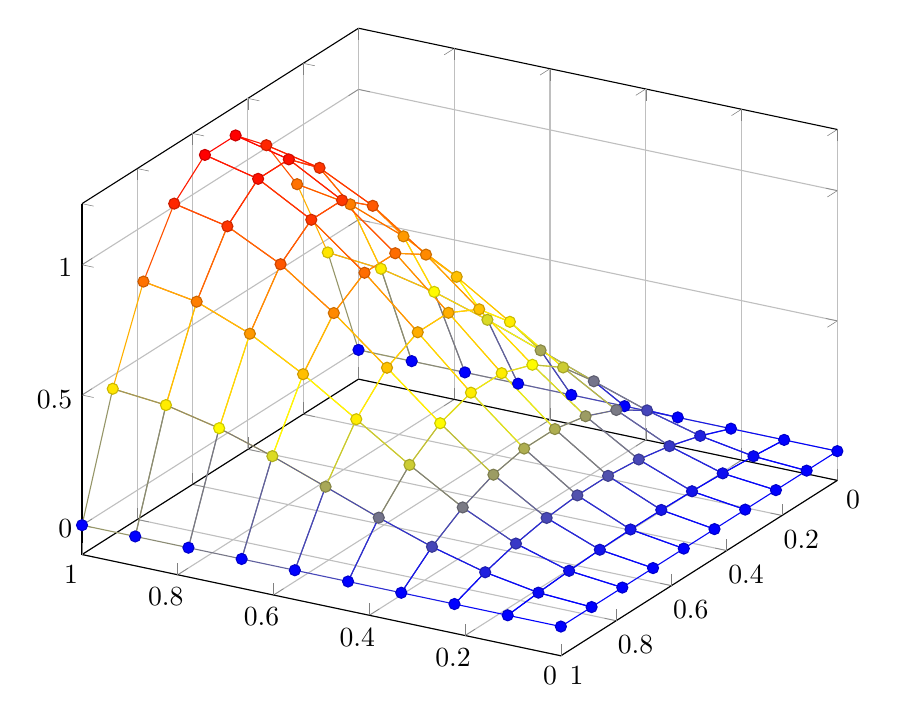
\begin{tikzpicture}
\begin{axis}[scale = 1.4, grid=major,view={210}{30}]
\addplot3+[mesh,scatter,samples=10,domain=0:1]{5*x*sin(2*deg(x)) * y*(1-y)};
\end{axis}
\end{tikzpicture}
\caption{An example finite elements mesh for the diffusion equation.}
\label{fig:finiteElementsMesh}
\end{figure}

\"Ozi\c{s} \textit{et al} \cite{burgerFiniteElement} take an approach of solving Burgers' by first applying the Hopf-Cole transformation \eqref{coleHopf}, then deploying the technique of finite elements to the diffusion equation \eqref{diffusionEq}. The initial condition is \eqref{initialCond1} and boundary conditions are homogeneous \eqref{boundConds1}. First, the linear space of all test functions will be represented by $H[0, 1]$, known as a Sobolev space. A Sobolev space means that the given test function, $\Phi(x) \in L^2[0, 1]$, and it's derivative exists in $L^2[0, 1]$ as well. Now integrate the product of the heat equation \eqref{diffusionEq} and some test function like so \[\int_{0}^{1} \Phi(x) (v_t - \kappa v_{xx}) \,\mathrm{d} x = 0.\] Next we end up with
\begin{align}
\int_{0}^{1} \left(\Phi(x) v_t + \kappa v_x \Phi_x\right)  \,\mathrm{d} x = \kappa \left(\Phi(1) v_x(1, t) - \Phi(0) v_x(0,t) \right), \label{weakFormHeatEq}
\end{align}
after integration by parts. Equation \eqref{weakFormHeatEq} will be considered the weak form of the heat equation \eqref{diffusionEq}. In order to approximate it, a Galerkin method will be applied.

The approximate solution will be of the form 
\begin{align}
\widetilde{v}(x,t) = \sum_{i = 1}^{N + 1} b_i(t) \Psi_i(x) \label{finiteElementApprox}
\end{align}
where $\Psi_i(x) \in H[0, 1] (1 \leq i \leq N + 1)$ are linearly independent trial basis functions and $b_i(t) (1 \leq i \leq N + 1)$ are the yet undetermined differentiable functions of time. According to the Galerkin method, the trial basis functions and the test basis functions are equal, so they may be swapped in \eqref{finiteElementApprox}. Now, \[\Phi(x) = \sum_{i = 1}^{N + 1} a_i \Phi_i(x),\] for every test function $\Phi(x)$, where $a_i (1 \leq i \leq N + 1)$ are arbitrary real numbers.

Divide the interval $[0, 1]$ up into $N$ subintervals $\Omega_1, \Omega_2, \dots, \Omega_N$ of $h_1, h_2, \dots, h_N$ respectively. The following is how the $i$th element (the line segment $\Omega_i$), will be denoted \[\Omega_i = [x_i, x_{i + 1}]; \quad\quad h_i = x_{i + 1} - x_i, \quad\quad \text{ for } i = 1, 2, \dots, N + 1.\] Now we can construct the test functions (see Figure \ref{fig:testFunctions})
\begin{align}
\label{hatFunctions}
\Phi_i(x) = \begin{cases} 
\frac{x - x_{i - 1}}{h_{i - 1}}, & x \in \Omega_{i - 1} \\
1 - \frac{x - x_i}{h_i}, & x \in \Omega_i \hspace{2cm} \text{ for } i = 1, 2, \dots, N + 1 \\
0, & x\notin \Omega_{i - 1} \cup \Omega_i
\end{cases}.
\end{align}
\begin{figure}[h!]
	\centering
	\resizebox{10cm}{!}{
	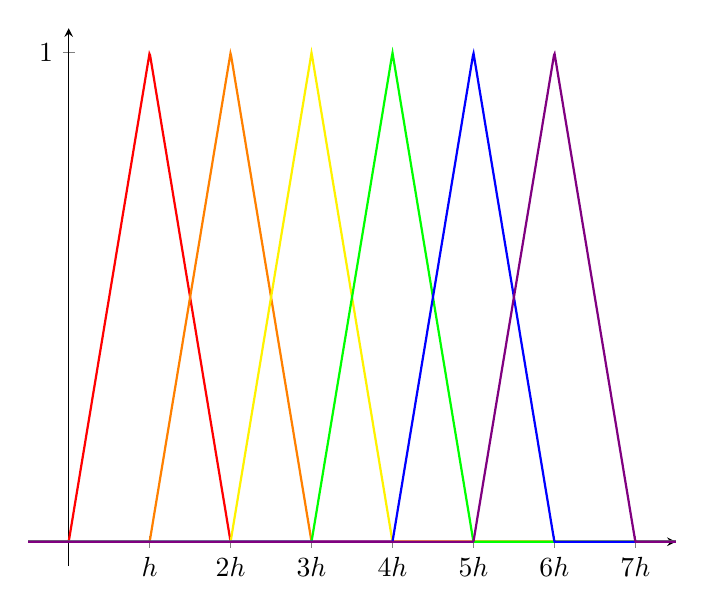
\begin{tikzpicture}[declare function = {
		f1(\x) = and(\x >= 0, \x < 2)*(\x/2) + and(\x >= 2, \x <= 4)*((4 - \x)/2);
		f2(\x) = and(\x >= 2, \x < 4)*((\x - 2)/2) + and(\x >= 4, \x <= 6)*((6 - \x)/2);
		f3(\x) = and(\x >= 4, \x < 6)*((\x - 4)/2) + and(\x >= 6, \x <= 8)*((8 - \x)/2);
		f4(\x) = and(\x >= 6, \x < 8)*((\x - 6)/2) + and(\x >= 8, \x <= 10)*((10 - \x)/2);
		f5(\x) = and(\x >= 8, \x < 10)*((\x - 8)/2) + and(\x >= 10, \x <= 12)*((12 - \x)/2);
		f6(\x) = and(\x >= 10, \x < 12)*((\x - 10)/2) + and(\x >= 12, \x <= 14)*((14 - \x)/2);}]
	\begin{axis}[scale = 1.2, axis x line = middle, axis y line = middle, ymin = -0.05, ymax = 1.05, ytick = {1}, xmin = -1,
	xmax = 15, xtick = {2, 4, 6, 8, 10, 12, 14}, xticklabels = {$h$, $2h$, $3h$, $4h$, $5h$, $6h$, $7h$}, domain = -1:15]
	\addplot[red,    thick] {f1(x)};
	\addplot[orange, thick] {f2(x)};
	\addplot[yellow, thick] {f3(x)};
	\addplot[green,  thick] {f4(x)};
	\addplot[blue,   thick] {f5(x)};
	\addplot[violet, thick] {f6(x)};
	\end{axis}
	\end{tikzpicture}}
	\caption{Piecewise linear functions}
	\label{fig:testFunctions}
\end{figure}

Plugging in the boundary conditions \eqref{boundConds1} into \eqref{weakFormHeatEq} we get
\begin{align}
\int_{0}^{1} \left(\Phi(x) v_t + \kappa v_x \Phi_x\right) \,\mathrm{d} x = 0. \label{weakFormHeatEq2}
\end{align}
Next 
\begin{align}
v_h(x, t) = \sum_{i = 1}^{N + 1} b_i(t) \Phi_i(x), \label{approxHeat}
\end{align}
where $v_h(x,t)$ is the approximate solution of the heat equation. Now plugging \eqref{approxHeat} into \eqref{weakFormHeatEq2} leaves us with 
\begin{align}
\int_{0}^{1} \left(\Phi(x) \frac{\partial v_h}{\partial t} (x, t) + \kappa \frac{\mathrm{d} \Phi}{\mathrm{d} x} \frac{\partial v_h}{\partial x}(x, t)\right) \,\mathrm{d} x = 0. \label{finiteElements1}
\end{align}
Next substitute \eqref{approxHeat} into \eqref{finiteElements1} and after some simplification, the system becomes \[\sum_{N + 1}^{i = 1} \sum_{N + 1}^{j = 1}a_i \left( \frac{\mathrm{d} b_j}{\mathrm{d} t} \int_{0}^{1} \Phi_i(x) \Phi_j(x) \,\mathrm{d} x \right) = - \sum_{N + 1}^{i = 1}\sum_{N + 1}^{j = 1} a_i \left(b_j \int_{0}^{1} \Phi_i'(x) \Phi_j'(x) \,\mathrm{d} x.\right)\] Now we get a system of discrete linear first-order differential equations 
\begin{align}
\sum_{j = 1}^{n + 1} c_{ij} \frac{\mathrm{d} b_j}{\mathrm{d} t} = - \kappa \sum_{j = 1}^{N + 1} b_j k_{ij} \label{finiteElements2}
\end{align}
where $c_{ij}$ and $k_{ij}$ represent the following integrals
\begin{align}
	c_{ij} &= \int_{0}^{1} \Phi_i(x) \Phi_j(x) \,\mathrm{d}x \label{cij}\\
	k_{ij} &= \int_{0}^{1} \Phi_i'(x) \Phi_j'(x) \,\mathrm{d}x \label{kij}
\end{align}
for $1 \leq i, j \leq N + 1.$ The matrix form of the system \eqref{finiteElements2} is 
\begin{align}
C \frac{\mathrm{d}}{\mathrm{d} t} \underline{b}(t) + \kappa K \underline{b}(t) = 0 \label{finiteElementsMtx}
\end{align}
where $C$ and $K$ are $N + 1 \times N + 1$ tridiagonal positive definite symmetric matrices and $\underline{b}^j$ denotes the finite difference approximation to the vector $b$. We can solve the ODE system \eqref{finiteElementsMtx} using finite differences. Similarly, the time derivative is approximated by \[\frac{\mathrm{d}}{\mathrm{d} t} \underline{b} = \frac{1}{\Delta t} (\underline{b}^{j + 1} - \underline{b}^j). \] Introducing a weight factor $\theta \in [0, 1]$ allows \"Ozi\c{s} \textit{et al} to rewrite the system in its most general form 
\begin{align}
	\frac{1}{\Delta t} C \left(\underline{b}^{j + 1} - \underline{b}^{j}\right) + \kappa K \left(\theta \underline{b}^{j + 1} + (1 - \theta)\underline{b}^{j}\right) = 0. \label{finiteElementSystem}
\end{align}

A rearrangement of the system then takes the form
\begin{align}
	D \underline{b}^{j + 1} = E \underline{b}^j \label{finiteElementEquation}
\end{align}
where
\begin{align*}
	D = C + \kappa \theta \Delta t K \quad\quad\quad \text{ and } \quad\quad\quad E = C - \kappa (1 - \theta) \Delta t K.
\end{align*}
Using the initial condition, this system can be solved. 

Once the system has been solved, the discretized Cole-Hopf transformation \eqref{coleHopfDiscrete} is used to establish an approximation to Burgers' equation. 

\subsection{My Implementation}

I coded the finite elements approach by following the work of \"Ozi\c{s} \textit{et al} \cite{burgerFiniteElement}. The following will contain some simplifications as well as some more detailed information regarding the approach.

First notice that the definition of the chosen piecewise linear functions \eqref{hatFunctions}, or hat functions, are made \textit{very} general. This is usually a strength of the finite element method because if gives the user a choice of picking the most appropriate function to cover a given subregion. For our purposes, since we are solving Burgers' equation on a rectangular domain, we can make simplifications to these hat functions. We will use equidistant points in the space domain, which implies the $h$ will no longer require a subscript, because every subinterval will be the same length. The corollary of this choice is that for each case of hat functions $\Phi_i$ and $\Phi_j$ such that $i = j$ and $|i - j| = 1$, these will all be equal.

Take the first hat function, $\Phi_1$, where \eqref{hatFunctions} implies that 
\begin{align}
	\label{hat1}
	\Phi_1(x) = \begin{cases} 
	\frac{x - x_{0}}{h}, & x \in \Omega_{0} \\
	1 - \frac{x - x_1}{h}, & x \in \Omega_1 \\
	0, & x\notin \Omega_{0} \cup \Omega_1.
	\end{cases}
\end{align}
Notice that on the interval $[0, L]$ we can find the values $x_0$ and $x_1$ quite easily. Since $x_i = ih$ this suggests that $x_0 = 0$ and $x_1 = h$. Next we have two integrals to compute, namely for the cases $i = j$ and $|i - j| = 1$. Because the hat functions have compact support, they are zero on most of the domain and hence the products of them for $|i - j| \geq 2$ will all be $0$. Now let us take the case of $i = j$ for the first piecewise linear function in the domain. The first step is to compute the product of $\Phi_i \Phi_i$ on the first region, $\Omega_0$, which is \[\Phi_1 \Phi_1 = \frac{x^2}{h^2}.\] Now computing the integral leaves us with \[\int_{0}^{h} \Phi_1 \Phi_1 \,\mathrm{d}x = \frac{x^3}{3 h^2} \Bigg|_{0}^{h} = \frac{h}{3}.\] As you can see in Figure \ref{fig:hatFunctions}, due to symmetry, the integral on the subsequent region, $\Omega_1$, will be $h/3$ also. Therefore, \[\int_{0}^{1} \Phi_1 \Phi_1 \,\mathrm{d}x = \int_{0}^{2h} \Phi_1 \Phi_1 \,\mathrm{d}x = \frac{2h}{3}.\]

\begin{figure}[h!]
	\centering
	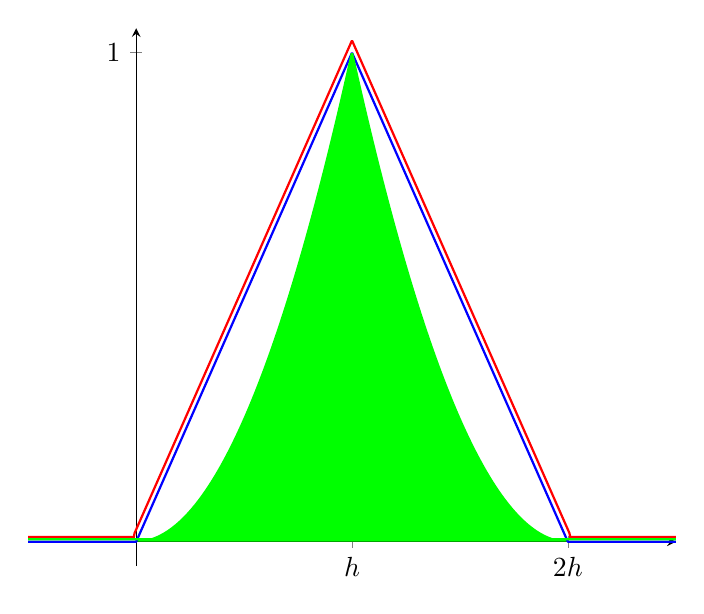
\begin{tikzpicture}[declare function = {
		f1(\x) = and(\x >= 0, \x < 2)*(\x/2) + and(\x >= 2, \x <= 4)*((4 - \x)/2);
		f2(\x) = (\x < -0.02)*(0.01) + and(\x >= -0.02, \x < 2)*((\x + 0.05)/2) + and(\x >= 2, \x <= 4.02)*((4.05 - \x)/2) + (\x > 4.02)*(0.01);
		f3(\x) = (\x < 0.1414)*(0.005) + and(\x >= 0.1414, \x < 2)*((\x^2)/4) + and(\x >= 2, \x <= 3.8585)*((16 - 8*\x + \x^2)/4) + (\x > 3.8585)*(0.005);
		f4(\x) = 0;}]
	\begin{axis}[scale = 1.2, axis x line = middle, axis y line = middle, ymin = -0.05, ymax = 1.05, ytick = {1}, xmin = -1,
	xmax = 5, xtick = {2, 4}, xticklabels = {$h$, $2h$}, domain = -1:5]
	\addplot[blue,  thick] {f1(x)};
	\addplot[red,   thick] {f2(x)};
	\addplot[green, thick, name path = A] {f3(x)};
	\addplot[draw = none,  name path = B] {f4(x)};
	\addplot[green] fill between[of = A and B, soft clip = {domain = 0:4}];
	\end{axis}
	\end{tikzpicture}
	\caption{The area under the curve of $\Phi_1 \Phi_1$}
	\label{fig:hatFunctions}
\end{figure}

Next for the $|i - j| = 1$ case, we introduce the following hat function in the sequence
\begin{align}
	\label{hat2}
	\Phi_2(x) = \begin{cases} 
	\frac{x - x_{1}}{h}, & x \in \Omega_1 \\
	1 - \frac{x - x_2}{h}, & x \in \Omega_2 \\
	0, & x\notin \Omega_{1} \cup \Omega_2,
	\end{cases}
\end{align}
and we know that $x_1 = h$ and $x_2 = 2h$. The product of $\Phi_1 \Phi_2$ on $\Omega_1$ is \[\Phi_1 \Phi_2 = \frac{1}{h^2} (x - h)(2h - x) = \frac{1}{h^2} (-x^2 + 3hx - 2h^2).\] Next we compute the integral over the same region, displayed in Figure \ref{fig:hatFunctions2} \[\int_{h}^{2h} \Phi_1 \Phi_2 \,\mathrm{d}x = \frac{1}{h^2} \left(-\frac{x^3}{3} + \frac{3hx^2}{2} - 2h^2 x\right) \Bigg|_{h}^{2h} = -\frac{8h}{3} + 6h - 4h - \left(- \frac{h}{3} + \frac{3h}{2} - 2h\right) = \frac{h}{6}.\] 

\begin{figure}[h!]
	\centering
	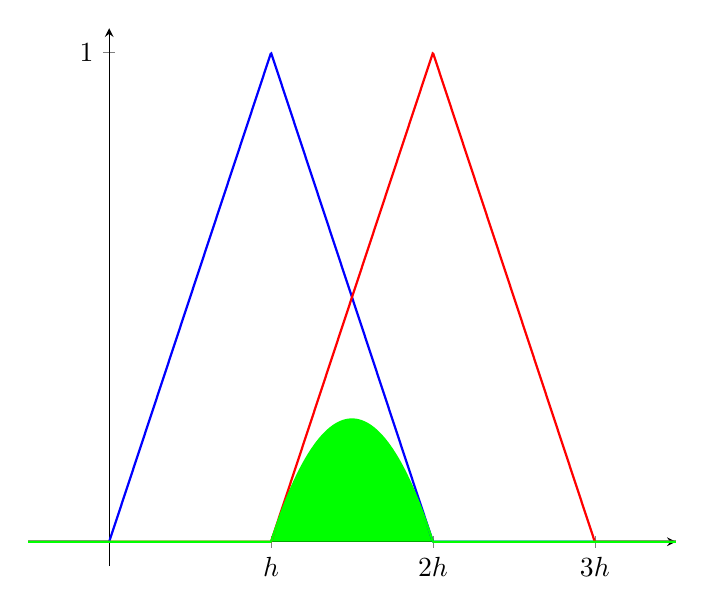
\begin{tikzpicture}[declare function = {
		f1(\x) = and(\x >= 0, \x < 2)*(\x/2) + and(\x >= 2, \x <= 4)*((4 - \x)/2);
		f2(\x) = and(\x >= 2, \x < 4)*((\x - 2)/2) + and(\x >= 4, \x <= 6)*((6 - \x)/2);
		f3(\x) = and(\x >= 2, \x < 4)*(((-1)*\x^2 + 6*\x - 8)/4);
		f4(\x) = 0;}]
	\begin{axis}[scale = 1.2, axis x line = middle, axis y line = middle, ymin = -0.05, ymax = 1.05, ytick = {1}, xmin = -1,
	xmax = 7, xtick = {2, 4, 6}, xticklabels = {$h$, $2h$, $3h$}, domain = -1:7]
	\addplot[blue,  thick] {f1(x)};
	\addplot[red,   thick] {f2(x)};
	\addplot[green, thick, name path = A] {f3(x)};
	\addplot[draw = none,  name path = B] {f4(x)};
	\addplot[green] fill between[of = A and B, soft clip = {domain = 2:4}];
	\end{axis}
	\end{tikzpicture}
	\caption{The area under the curve of $\Phi_1 \Phi_2$}
	\label{fig:hatFunctions2}
\end{figure}

It follows from this result that we can calculate all the constants, $c_{ij}$, for $1 \leq i, j \leq N + 1.$ Therefore we can construct the following tridiagonal matrix
\begin{align}
\label{C}
C = 
\begin{bmatrix}
\frac{2h}{3} & \frac{h}{6} &&&&& \\
\frac{h}{6} & \frac{2h}{3} & \frac{h}{6} &&&& \\
&&& \ddots &&& \\
&&&& \frac{h}{6} & \frac{2h}{3} & \frac{h}{6} \\
&&&&& \frac{h}{6} & \frac{2h}{3}
\end{bmatrix}.
\end{align}

Next we must compute the $k_{ij}$ constants. In order to do this, we require derivatives of \eqref{hat1} and \eqref{hat2} as follows
\begin{align*}
	\Phi_i'(x) = 
	\begin{cases} 
	\frac{1}{h}, & x \in \Omega_{i - 1} \\
	- \frac{1}{h}, & x \in \Omega_i \\
	0, & x\notin \Omega_{i - 1} \cup \Omega_i
	\end{cases} 
\end{align*}
for each $i = 1, 2, \dots, N + 1.$ The calculation for $k_{ij}$ in the cases $i = j$ and $|i - j| = 1$ are both given below (see Figure \ref{fig:hatFunctions3})
\begin{align*}
	\int_{0}^{1} \Phi_1' \Phi_1' \,\mathrm{d} x &= 2 \int_{0}^{h} \frac{1}{h^2} \,\mathrm{d} x = \frac{2}{h} \\
	\int_{0}^{1} \Phi_1' \Phi_2' \,\mathrm{d} x &= \int_{h}^{2h} -\frac{1}{h^2} \,\mathrm{d} x = -\frac{1}{h}.
\end{align*}
Now we can construct our next matrix,
\begin{align}
\label{K}
K = 
\begin{bmatrix}
\frac{2}{h} & -\frac{1}{h} &&&&& \\
-\frac{1}{h} & \frac{2}{h} & -\frac{1}{h} &&&& \\
&&& \ddots &&& \\
&&&& -\frac{1}{h} & \frac{2}{h} & -\frac{1}{h} \\
&&&&& -\frac{1}{h} & \frac{2}{h}
\end{bmatrix}.
\end{align}
\begin{figure}[h!]
	\centering
	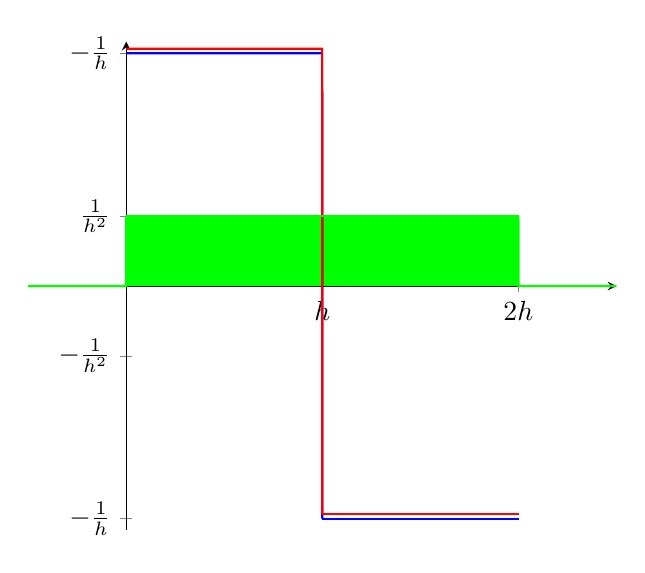
\begin{tikzpicture}[declare function = {
		f1(\x) = and(\x >= 0, \x < 2)*(1) + and(\x >= 2, \x <= 4)*(-1);
		f2(\x) = and(\x >= 0, \x < 2)*(1.02) + and(\x >= 2, \x <= 4)*(-0.98);
		f3(\x) = and(\x >= 0, \x <= 4)*(0.3);
		f4(\x) = 0;}]
	\begin{axis}[scale = 1.09, axis x line = middle, axis y line = middle, ymin = -1.05, ymax = 1.05, ytick = {-1, -0.3, 0.3, 1}, yticklabels = {$-\frac{1}{h}$, $-\frac{1}{h^2}$, $\frac{1}{h^2}$, $-\frac{1}{h}$}, xmin = -1, xmax = 5, xtick = {2, 4}, xticklabels = {$h$, $2h$}, domain = -1:5]
	\addplot[blue,  thick, domain =  0:2] {f1(x)};
	\addplot[blue,  thick, domain =  2:4] {f1(x)};
	\addplot[red,   thick, domain =  0:2] {f2(x)};
	\addplot[red,   thick, domain =  2:4] {f2(x)};
	\addplot[green, thick, domain = -1:0] {f3(x)};
	\addplot[green, thick, domain =  0:4, name path = A] {f3(x)};
	\addplot[green, thick, domain =  4:5] {f3(x)};
	\addplot[draw  = none, name path = B] {f4(x)};
	\addplot[green] fill between[of = A and B, soft clip = {domain = 0:4}];
	\end{axis}
	\end{tikzpicture}
	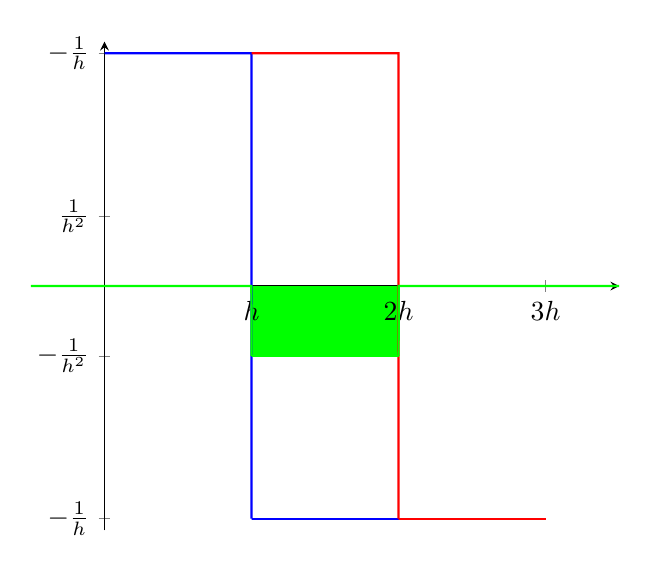
\begin{tikzpicture}[declare function = {
		f1(\x) = and(\x >= 0, \x < 2)*(1) + and(\x >= 2, \x <= 4)*(-1);
		f2(\x) = and(\x >= 2, \x < 4)*(1) + and(\x >= 4, \x <= 6)*(-1);
		f3(\x) = and(\x >= 2, \x <= 4)*(-0.3);
		f4(\x) = 0;}]
	\begin{axis}[scale = 1.09, axis x line = middle, axis y line = middle, ymin = -1.05, ymax = 1.05, ytick = {-1, -0.3, 0.3, 1}, yticklabels = {$-\frac{1}{h}$, $-\frac{1}{h^2}$, $\frac{1}{h^2}$, $-\frac{1}{h}$}, xmin = -1, xmax = 7, xtick = {2, 4 , 6}, xticklabels = {$h$, $2h$, $3h$}, domain = -1:7]
	\addplot[blue,  thick, domain =  0:2] {f1(x)};
	\addplot[blue,  thick, domain =  2:4] {f1(x)};
	\addplot[red,   thick, domain =  2:4] {f2(x)};
	\addplot[red,   thick, domain =  4:6] {f2(x)};
	\addplot[green, thick, domain = -1:2] {f3(x)};
	\addplot[green, thick, domain =  2:4, name path = A] {f3(x)};
	\addplot[green, thick, domain =  4:7] {f3(x)};
	\addplot[draw  = none, name path = B] {f4(x)};
	\addplot[green] fill between[of = A and B, soft clip = {domain = 2:4}];
	\end{axis}
	\end{tikzpicture}
	\caption{The area under the curve of $\Phi_1' \Phi_1'$ (\textit{left}) and $\Phi_1' \Phi_2'$ (\textit{right}).}
	\label{fig:hatFunctions3}
\end{figure}

At this point we have now established \eqref{finiteElementsMtx}. With an introduction of the finite difference approximation to the time derivatives and the weight factor $\theta$, the system becomes \eqref{finiteElementSystem}. The system can undergo another change into \eqref{finiteElementEquation}. From this form a solution to the Diffusion equation can be established. Then, the discrete Cole-Hopf transformation \eqref{coleHopfDiscrete} is used to arrive at the solution we seek.

Algorithm \ref{alg:FiniteElements} is the pseudocode I used to deploy the finite element method. The initial condition will be $j = 0$, \[v_{_{i, 0}} = \exp \left(- \frac{1}{2 \kappa} \int_{0}^{x} \psi(s) \,\mathrm{d} s \right).\] 

\begin{algorithm}[h!]
	\SetKwInOut{Input}{Input}
	\SetKwInOut{Output}{Output}
	\underline{function FiniteElements} $(f, \kappa, L, T, N, M, \theta)$\;
	\Input{The initial condition, $f$, the viscosity coefficient, $\kappa$, the length of the space interval, $L$, the length of the time interval, $T$, the number of sub-intervals in space, $N$, the number of sub-intervals in time, $M$, and the weight factor, $\theta$}
	\Output{The solution to the diffusion equation, $v$, as a matrix of points}
	$h = L/N$; \tcp{Set the mesh width for space}
	$k = T/M$; \tcp{Set the mesh width for time}
	\For{$i = 0$ \KwTo $N$}
	{
		$v_{_{i, 0}} = f(ih)$; \tcp{Compute the solution for the first time step, $j = 0$}
	}
	Build the tridiagonal matrix $C$, (see above)\;
	Build the tridiagonal matrix $K$, (see above)\;
	$D = C + \kappa \theta k K$; \tcp{Construct the matrix D}
	$E = C - \kappa (1 - \theta) k K$; \tcp{Construct the matrix E}
	\For{$j = 0$ \KwTo $M - 1$}
	{
		\tcc{Solve the system of equations for the next time step.}
		$v_{_{:, j + 1}} = D \textbackslash(E\,v_{_{:, j}})$ \tcp{Fill the $j + 1$-th column of the solution matrix $v$}
	}
	\caption{Finite Elements Scheme for the Diffusion Equation}
	\label{alg:FiniteElements}
\end{algorithm}

\section{Spectral Methods}

Spectral methods are a technique that incorporate Fourier transforms to move the given functions into the frequency-domain, which in turn allows for easier computation. In particular the use of the Fast Fourier Transform (FFT) creates a solution in terms of a sum of sinusoidal functions. The final step is to choose the coefficients of these basis functions which satisfy the PDE.

Basdevant \textit{et al} \cite{burgerSpectral} worked on several spectral methods in their paper. First to set up the question, they chose the following initial and boundary conditions
\begin{subequations}
	\label{spectralMethodConds}
	\begin{align}
	u(x, 0) &= -\sin \pi x, \quad |x| \leq 1 \label{initialCond4} \\
	u(\pm 1, 0) &= 0 \label{boundConds4}.
	\end{align}
\end{subequations}
Basdevant \textit{et al} make a interesting change of variables, namely they substitute $x' = \pi x$ and $t' = \pi t$, then drop the primes, which means $x'$ and $t'$ will be displayed as $x$ and $t$, respectively. The problem \eqref{spectralMethodConds} changes slightly to the following
\begin{align*}
u_t + uu_x &= \kappa' u_{xx}, \quad -\pi \leq x \leq \pi, \quad t >0 \\
u(x, 0) &= - \sin x,
\end{align*}
where $\kappa' = \pi \kappa.$ A truncated Fourier series can now approximate the solution because it is $2\pi$-periodic. This is represented as 
\begin{align*}
u_n(x, t) = \sum_{k = - N}^{N} u_k(t)e^{ikx}.
\end{align*} 
Basdevant \textit{et al} cite Gottlieb and Orszag \cite{spectralMethod} with coming up with the following spectral equations
\begin{align}
\frac{\mathrm{d} u_k}{\mathrm{d} t} = -\frac{ik}{2} N_k(\textbf{u}, \textbf{u}) - \kappa'k^2 u_k, \quad -N \leq k \leq N, \label{spectralMethod1}
\end{align}
with the initial conditions
\begin{align*}
u_k(0) &= 0 &\text{ for } k & \neq 1 \\
u_t(0) &= i/2 & u_{-1}(0) &= -i/2,
\end{align*}
where $\textbf{u} = [u_k]$ and $N_k(\textbf{u}, \textbf{u})$ represents nonlinear term which follows from the convolution product.

Now assume $M \geq N$ and set the following parameters
\begin{align*}
\widetilde{u_k} & = u_k & |k| &\leq N \\
\widetilde{u_k} & = 0 & N & < |k| \leq M.
\end{align*}
Next, Basdevant \textit{et al} set out the following algorithm:

\begin{algorithm}
	Perform an in inverse Discrete Fourier Transform (DFT) using Fast Fourier algorithm (FFT) of length $M$ on $\widetilde{u_k}$ to obtain $u(x_j), x_j = 2 \pi j / 2M, 0 \leq j \leq 2M - 1$\;
	Compute $w(x_j) = u(x_j)^2, 0 \leq j \leq 2M - 1$\;
	Perform the direct DFT of length $M$ on the $w(x_j)$ values to produce $u * u(k) = w_k, - M \leq k \leq M$\;
	\caption{Computing the Discrete Fourier Transform (DFT)}
\end{algorithm}
The DFT will convert the problem into the frequency domain where algebraic manipulations can be performed.

The scheme is the Galerkin method if $M > \frac{3}{2} N$ and \[N_k(\textbf{u}, \textbf{u}) = \sum_{p = - N}^{N} u_p u_{k - p}.\] On the other hand, the pseudo-spectral scheme is
\begin{align*}
N_k(\textbf{u}, \textbf{u}) =& \sum u_pu_q, \\
& |p|, |q| \leq N \\
& k = p + q + 2Me,
\end{align*}
when $\frac{3}{2}N \geq M \geq N$, where $e$ may be 0 or $\pm 1$. 

Next, rewrite \eqref{spectralMethod1} as \[\frac{\mathrm{d} u_k}{\mathrm{d} t} = \mathcal{N}_k (\textbf{u}, \textbf{u})+ \lambda u_k, \quad\quad\quad \mathcal{N}_k = -\frac{ik}{2}N_k,\]
\begin{align} 
\lambda = - \kappa'k^2. \label{lambda}
\end{align}
Integrating \eqref{lambda} with respect to time yields \[u_k(t + \Delta t) = u_k(t - \Delta t) e^{2\lambda \Delta t} + \int_{t - \Delta t}^{t + \Delta t} \mathcal{N}_k(\textbf{u}, \textbf{u})(\tau)e^{\lambda(t + \Delta t - \tau)} \, \mathrm{d} \tau.\] Finally, applying the trapezoidal rule gives the final explicit equation for the spectral method
\begin{align*}
u_k(t + \Delta t) = u_k (t - \Delta t)e^{2 \lambda \Delta t} + 2 \Delta t e{\lambda \Delta t} \mathcal{N}_k (\textbf{u}, \textbf{u})(t).
\end{align*}

\chapter{Results}
\label{sec:results}

This section will be comprised of a quantitative and qualitative review of the analytical solution and numerical methods developed as part of this project. First the graphs of the analytic solution to the viscous Burgers' equation will be presented and commented on. Then the rest of the section will focus on the numerical methods, in this case the finite differences and finite elements schemes.

The computer code that I used to produce the following images and tables is presented in Appendix \ref{sec:code}. An example of how one would implement each function is given in Listing \ref{code:test}.

\section{Analytical Solution}

Graphs of the analytical solution are produced using the code from Listing \ref{code:analyticalSoln} and the code for applying the Cole-Hopf transformation is provided in Listing \ref{code:ColeHopf}. 

The graphs and tables throughout this section will be based on one of two initial conditions. For clarity we will define the following sinusoidal initial condition as initial condition 1 \[u(x, 0) = \sin (\pi x), \quad 0 \leq x \leq 1.\] The remaining condition is \[u(x, 0) = 4x(1 - x), \quad 0 \leq x \leq 1,\] and this parabolic equation will be referred to as initial condition 2. The spatial domain will be of unit length, which means $L = 1$, so therefore $x \in [0, 1]$. Usually the temporal domain is given by $[0, \tau]$. For most of the following cases, a choice of $\tau$ is arbitrary and just done so the graphs are displayed nicely. Different values of $\tau$ will be used in the data portion of this chapter however.

Following the last image will be explanations and a discussion (see Figures \ref{fig:solnBurgers1} - \ref{fig:solnBurgersTimePlot2}).

\begin{figure}[h!]
	\centering
	\includegraphics[width=14.5cm, trim = {160 0 150 0} ]{Figures/solnBurgers1.png}
	\caption{The approximated analytical solution of Burgers' equation with $Re = 1$ for initial conditions 1 and 2 on the left and right respectively.}
	\label{fig:solnBurgers1}
\end{figure}

\begin{figure}[h!]
	\centering
	\includegraphics[width=14.5cm, trim = {160 0 150 0} ]{Figures/solnBurgers2.png}
	\caption{The approximated analytical solution of Burgers' equation with $Re = 5$ for initial conditions 1 and 2 on the left and right respectively.}
	\label{fig:solnBurgers2}
\end{figure}

\begin{figure}[h!]
	\centering
	\includegraphics[width=14.5cm, trim = {160 0 150 0} ]{Figures/solnBurgers3.png}
	\caption{The approximated analytical solution of Burgers' equation with $Re = 15$ for initial conditions 1 and 2 on the left and right respectively.}
	\label{fig:solnBurgers3}
\end{figure}

\begin{figure}[h!]
	\centering
	\includegraphics[width=14.5cm, trim = {160 0 150 0} ]{Figures/solnBurgers4.png}
	\caption{The approximated analytical solution of Burgers' equation with $Re = 55$ for initial conditions 1 and 2 on the left and right respectively.}
	\label{fig:solnBurgers4}
\end{figure}

\begin{figure}[h!]
	\centering
	\includegraphics[width=14.5cm, trim = {160 0 150 0} ]{Figures/BurgersVsDiffusion1.png}
	\caption{For a $Re = 1$, on the left is the approximated analytical solution of Burgers' equation with initial conditions 1 and on the right is the corresponding approximated analytical solution of the diffusion equation with $v(x, 0) = \exp\left(\frac{\cos(\pi x) - 1}{2 \kappa \pi}\right)$.}
	\label{fig:BurgersVsDiffusion1}
\end{figure}

\begin{figure}[h!]
	\centering
	\includegraphics[width=14.5cm, trim = {160 0 150 0} ]{Figures/BurgersVsDiffusion2.png}
	\caption{For a $Re = 20$, on the left is the approximated analytical solution of Burgers' equation with initial conditions 1 and on the right is the corresponding approximated analytical solution of the diffusion equation with $v(x, 0) = \exp\left(\frac{\cos(\pi x) - 1}{2 \kappa \pi}\right)$.}
	\label{fig:BurgersVsDiffusion2}
\end{figure}

\begin{figure}[h!]
	\centering
	\includegraphics[width=14.5cm, trim = {160 0 150 0} ]{Figures/BurgersVsDiffusionV2_1.png}
	\caption{For a $Re = 1$, on the left is the approximated analytical solution of Burgers' equation with initial conditions 1 and on the right is the approximated analytical solution of the diffusion equation with initial condition 1 as well.}
	\label{fig:BurgersVsDiffusionV2_1}
\end{figure}

\begin{figure}[h!]
	\centering
	\includegraphics[width=14.5cm, trim = {160 0 150 0} ]{Figures/BurgersVsDiffusionV2_2.png}
	\caption{For a $Re = 40$, on the left is the approximated analytical solution of Burgers' equation with initial conditions 1 and on the right is the approximated analytical solution of the diffusion equation with initial condition 1 as well.}
	\label{fig:BurgersVsDiffusionV2_2}
\end{figure}

\begin{figure}[h!]
	\centering
	\includegraphics[width=14.5cm, trim = {160 0 150 0} ]{Figures/solnBurgersTimePlot1.png}
	\caption{The approximated analytical solution of Burgers' equation at various times $t$, with $Re = 1$ for initial conditions 1 and 2 on the left and right respectively.}
	\label{fig:solnBurgersTimePlot1}
\end{figure}

\begin{figure}[h!]
	\centering
	\includegraphics[width=14.5cm, trim = {160 0 150 0} ]{Figures/solnBurgersTimePlot2.png}
	\caption{The approximated analytical solution of Burgers' equation at various times $t$, with $Re = 55$ for initial conditions 1 and 2 on the left and right respectively.}
	\label{fig:solnBurgersTimePlot2}
\end{figure}
\clearpage

First we see in Figures \ref{fig:solnBurgers1} through to \ref{fig:solnBurgers4}, the surface plot of the analytical solution of the Viscous Burgers' equation. In order, these plots are computed with a Reynolds number of $Re = 1, 5, 15,$ and $55$. For this level of viscosity, we notice that the sinusoidal and parabolic initial conditions are indistinguishable from one another. Another common behaviour for each of the plots is that the solution converges to 0 as time increases. An increase of the Reynolds number represents more turbulent flows, and as expected, the solution dissipates more slowly. The curious behavior is the fact that the crest of the wave travels away from the initial position. This characteristic is a primitive feature of shock formation; it is primitive because the Reynolds number is still quite small, but nonetheless, the solution still dissipates and converges to 0. This behaviour is due to the nature of Burgers' equation as it represents a fluid that has negligible change in pressure internally within the fluid. This basically means that the particles of fluid are not showing signs of applying forces to one another that might manifest as sporadic behaviour. Instead, Burgers' equation models a fluid that is, let us say, ``well behaved,'' and flows smoothly.

Recall that the initial condition of the diffusion equation is a Cole-Hopf transformation of the original sine initial condition of Burgers' equation (See Figures \ref{fig:BurgersVsDiffusion1} \& \ref{fig:BurgersVsDiffusion2}). Clearly the curve at $t = 0$ behaves as an exponential function, which is to be expected. A big difference between the two plots is that the diffusion equation does not approach 0 as time increases, which is what Burgers' equation does. Instead, the solution to the diffusion equation seems to approach 8.5 approximately; this seems like it could be the average of the initial condition. The physical meaning of the diffusion equation is that given some initial profile of heat, the heat should diffuse into the rest of the domain as time gets larger. In other words, the amount of heat energy at the initial time will be conserved (because energy is conserved), such that as time gets large, the temperature in every position is uniform. Notice in Figure \ref{fig:BurgersVsDiffusion2} that the increase in the Reynolds number shifts the initial condition vertically downwards, which effects the average function value. In addition, the diffusion process is occurring more slowly.

The final two surface plots depict the solution of Burgers' equation and the heat equation given initial condition 1. Both Figure \ref{fig:BurgersVsDiffusionV2_1} \& \ref{fig:BurgersVsDiffusionV2_2} clearly have exactly the same initial condition. Despite the different values for the dissipation coefficient in each of the plots, the heat equation converges to the same value for both graphs. The explanation is that the initial condition for both cases is the same, and thus the average function value is the same. The average function value is computed as follows \[f_{avg} = \frac{1}{b - a} \int_{a}^{b} f(x) \,\mathrm{d}x = \frac{1}{1 - 0} \int_{0}^{1} \sin (\pi x) \,\mathrm{d} x = \frac{2}{\pi} \approx 0.636619.\] This calculation matches the value of which the solution to the diffusion equation is approaching as time increases.

The last two graphs regarding the analytical solution of Burgers' equation are Figures \ref{fig:solnBurgersTimePlot1} \& \ref{fig:solnBurgersTimePlot2}. Instead of a surface plot, the graphs depict univariate functions. In our case this shows the solution of Burgers' equation for initial conditions 1 and 2, plotted against the position. On the same graph, several different instances of time are shown so that we can more clearly see how the solution evolves over time. In Figure \ref{fig:solnBurgersTimePlot1} the Reynolds number is 1, so the solution just dissipates while the centre is fixed in space. Next, Figure \ref{fig:solnBurgersTimePlot2} shows us how the crest of the wave is travelling away from the initial position. This is the beginning of a shock formation. Due to the shape of this wave at $t = 0.40$, it is commonly refereed to as a triangle wave. It is a rather famous plot associated with Burgers' equation. 

Before moving on to numerical methods, an important question to ask is ``when would shock formation occur in a real life scenario?'' To answer this question, we must first introduce a concept called the Mach number.

The Mach number ($Ma$) is defined by the following \[Ma = \frac{u}{c}\] where $c$ is the speed of sound in some medium and $u$ is the flow velocity. This quantity is a ratio of some velocity to the speed of sound. For instance, if $u$ were to equal the speed of sound, then $u$ would be describe as travelling at Mach 1 because $Ma = 1.$ To quantify this value, the speed of sound through air at 20 \textdegree C is approximately 343 m/s. Supersonic speeds would refer to velocities that exceed Mach 1.

Shock formation occurs when the flow speed of some fluid is supersonic. Realistically in fluid dynamics, this behaviour would be exhibited by gases (as opposed to liquids---but in principle they are technically not excluded).

When a given initial condition is discontinuous, then shock formation may also occur. Similar characteristics could be observed in a liquid, if discontinuous initial conditions could be mimicked. This could plausibly be done by a container, or even an object obstructing the path of the fluid.

\section{Numerical Methods}

We now turn our focus to a discussion of numerical methods, and how well they compared to the approximated analytical solution. This section begins with the finite differences method and will be concluded with finite elements.

\subsection{Finite Differences}
\label{sec:FiniteDifferences}

First, Tables \ref{tab:error1} - \ref{tab:error6} will be used to report differences in the computation of the numerical method. Images of the absolute error with respect to the solution will follow in Figures \ref{fig:finiteDiffError1} - \ref{fig:finiteDiffError4}. The discussion will be presented after the images.

\begin{table}[!h]%H
	\centering
	\begin{threeparttable}
		\caption{Absolute error in the finite difference approximation for initial condition 1, with $\kappa = 1$ ($Re = 1$), $\tau = 0.1$, and $\Delta t = 0.001$}
		\label{tab:error1}
		\begin{tabular}{p{.13\linewidth} p{.15\linewidth} p{.15\linewidth} p{.15\linewidth} p{.15\linewidth} p{.1\linewidth}}
			\toprule
			$x$ & \multicolumn{5}{c}{Computed error for different values of $N$} \\
			\cmidrule{2-6}
		   	& $N = 10$ & $N = 20$ & $N = 40$ & $N = 80$ & $N = 160$\\
			\midrule
			0.1 & 0.000906 & 0.000226 & 0.000057 & 0.000015 & 0.000005 \\
			0.2 & 0.001738 & 0.000434 & 0.000110 & 0.000029 & 0.000009 \\
			0.3 & 0.002425 & 0.000606 & 0.000154 & 0.000041 & 0.000012 \\
			0.4 & 0.002900 & 0.000725 & 0.000183 & 0.000048 & 0.000014 \\
			0.5 & 0.003110 & 0.000777 & 0.000196 & 0.000051 & 0.000015 \\
			0.6 & 0.003018 & 0.000753 & 0.000190 & 0.000049 & 0.000014 \\
			0.7 & 0.002615 & 0.000652 & 0.000164 & 0.000042 & 0.000012 \\
			0.8 & 0.001928 & 0.000481 & 0.000121 & 0.000031 & 0.000009 \\
			0.9 & 0.001024 & 0.000255 & 0.000064 & 0.000016 & 0.000005 \\
			\bottomrule
		\end{tabular}
	\end{threeparttable}
\end{table}

\begin{table}[!h]%H
	\centering
	\begin{threeparttable}
		\caption{Absolute error in the finite difference approximation for initial condition 1, with $\kappa = 0.066666$ ($Re = 15$), $\tau = 0.1$, and $\Delta t = 0.001$}
		\begin{tabular}{p{.13\linewidth} p{.15\linewidth} p{.15\linewidth} p{.15\linewidth} p{.15\linewidth} p{.1\linewidth}}
			\toprule
			$x$ & \multicolumn{5}{c}{Computed error for different values of $N$}\\
			\cmidrule{2-6}
			& $N = 10$ & $N = 20$ & $N = 40$ & $N = 80$ & $N = 160$ \\
			\midrule
			0.1 & 0.014794 & 0.003655 & 0.000911 & 0.000228 & 0.000057 \\
			0.2 & 0.022725 & 0.005690 & 0.001423 & 0.000356 & 0.000089 \\
			0.3 & 0.019162 & 0.004898 & 0.001231 & 0.000308 & 0.000077 \\
			0.4 & 0.003048 & 0.000852 & 0.000219 & 0.000055 & 0.000013 \\
			0.5 & 0.022658 & 0.005799 & 0.001458 & 0.000365 & 0.000092 \\
			0.6 & 0.050970 & 0.013174 & 0.003322 & 0.000832 & 0.000208 \\
			0.7 & 0.071358 & 0.018352 & 0.004622 & 0.001157 & 0.000289 \\
			0.8 & 0.072042 & 0.018270 & 0.004583 & 0.001147 & 0.000286 \\
			0.9 & 0.046133 & 0.011520 & 0.002878 & 0.000719 & 0.000180 \\
			\bottomrule
		\end{tabular}
	\end{threeparttable}
\end{table}

\begin{table}[!h]%H
	\centering
	\begin{threeparttable}
		\caption{Absolute error in the finite difference approximation for initial condition 1, with $\kappa = 0.066666$ ($Re = 15$), $\tau = 0.01$, and $\Delta t = 0.001$}
		\begin{tabular}{p{.13\linewidth} p{.15\linewidth} p{.15\linewidth} p{.15\linewidth} p{.15\linewidth} p{.1\linewidth}}
			\toprule
			$x$ & \multicolumn{5}{c}{Computed error for different values of $N$} \\
			\cmidrule{2-6}
			& $N = 10$ & $N = 20$ & $N = 40$ & $N = 80$ & $N = 160$ \\
			\midrule
			0.1 & 0.173972 & 0.007713 & 0.002060 & 0.000516 & 0.000129 \\
			0.2 & 0.344758 & 0.009959 & 0.002699 & 0.000676 & 0.000169 \\
			0.3 & 0.502989 & 0.004394 & 0.001324 & 0.000330 & 0.000082 \\
			0.4 & 0.630404 & 0.006816 & 0.001497 & 0.000376 & 0.000095 \\
			0.5 & 0.702953 & 0.018272 & 0.004377 & 0.001097 & 0.000275 \\
			0.6 & 0.699441 & 0.024665 & 0.005976 & 0.001497 & 0.000374 \\
			0.7 & 0.611716 & 0.023865 & 0.005780 & 0.001446 & 0.000361 \\
			0.8 & 0.449751 & 0.017505 & 0.004225 & 0.001055 & 0.000264 \\
			0.9 & 0.236977 & 0.008852 & 0.002130 & 0.000531 & 0.000133 \\
			\bottomrule
		\end{tabular}
	\end{threeparttable}
\end{table}

\begin{table}[!h]%H
	\centering
	\begin{threeparttable}
		\caption{Absolute error in the finite difference approximation for initial condition 2, with $\kappa = 1$ ($Re = 1$), $\tau = 0.1$, and $\Delta t = 0.001$}
		\begin{tabular}{p{.13\linewidth} p{.15\linewidth} p{.15\linewidth} p{.15\linewidth} p{.15\linewidth} p{.1\linewidth}}
			\toprule
			$x$ & \multicolumn{5}{c}{Computed error for different values of $N$} \\
			\cmidrule{2-6}
			& $N = 10$ & $N = 20$ & $N = 40$ & $N = 80$ & $N = 160$ \\
			\midrule
			0.1 & 0.000929 & 0.000232 & 0.000059 & 0.000016 & 0.000005 \\
			0.2 & 0.001785 & 0.000446 & 0.000113 & 0.000030 & 0.000009 \\
			0.3 & 0.002496 & 0.000624 & 0.000158 & 0.000042 & 0.000013 \\
			0.4 & 0.002991 & 0.000747 & 0.000189 & 0.000050 & 0.000015 \\
			0.5 & 0.003212 & 0.000802 & 0.000203 & 0.000053 & 0.000016 \\
			0.6 & 0.003119 & 0.000778 & 0.000196 & 0.000051 & 0.000015 \\
			0.7 & 0.002703 & 0.000674 & 0.000170 & 0.000044 & 0.000012 \\
			0.8 & 0.001992 & 0.000497 & 0.000125 & 0.000032 & 0.000009 \\
			0.9 & 0.001057 & 0.000264 & 0.000066 & 0.000017 & 0.000005 \\
			\bottomrule
		\end{tabular}
	\end{threeparttable}
\end{table}

\begin{table}[!h]%H
	\centering
	\begin{threeparttable}
		\caption{Absolute error in the finite difference approximation for initial condition 2, with $\kappa = 0.066666$ ($Re = 15$), $\tau = 0.1$, and $\Delta t = 0.001$}
		\begin{tabular}{p{.13\linewidth} p{.15\linewidth} p{.15\linewidth} p{.15\linewidth} p{.15\linewidth} p{.1\linewidth}}
			\toprule
			$x$ & \multicolumn{5}{c}{Computed error for different values of $N$} \\
			\cmidrule{2-6}
			& $N = 10$ & $N = 20$ & $N = 40$ & $N = 80$ & $N = 160$ \\
			\midrule
			0.1 & 0.017010 & 0.004141 & 0.001029 & 0.000257 & 0.000065 \\
			0.2 & 0.024796 & 0.006236 & 0.001561 & 0.000390 & 0.000098 \\
			0.3 & 0.018704 & 0.004847 & 0.001223 & 0.000306 & 0.000076 \\
			0.4 & 0.000417 & 0.000045 & 0.000007 & 0.000002 & 0.000001 \\
			0.5 & 0.027630 & 0.007142 & 0.001801 & 0.000451 & 0.000113 \\
			0.6 & 0.055343 & 0.014321 & 0.003613 & 0.000905 & 0.000226 \\
			0.7 & 0.074181 & 0.019016 & 0.004784 & 0.001198 & 0.000299 \\
			0.8 & 0.074236 & 0.018751 & 0.004699 & 0.001175 & 0.000294 \\
			0.9 & 0.048359 & 0.012055 & 0.003010 & 0.000752 & 0.000188 \\
			\bottomrule
		\end{tabular}
	\end{threeparttable}
\end{table}

\begin{table}[!h]%H
	\centering
	\begin{threeparttable}
		\caption{Absolute error in the finite difference approximation for initial condition 2, with $\kappa = 0.066666$ ($Re = 15$), $\tau = 0.01$, and $\Delta t = 0.001$}
		\label{tab:error6}
		\begin{tabular}{p{.13\linewidth} p{.15\linewidth} p{.15\linewidth} p{.15\linewidth} p{.15\linewidth} p{.1\linewidth}}
			\toprule
			$x$ & \multicolumn{5}{c}{Computed error for different values of $N$} \\
			\cmidrule{2-6}
			& $N = 10$ & $N = 20$ & $N = 40$ & $N = 80$ & $N = 160$ \\
			\midrule
			0.1 & 0.195240 & 0.010842 & 0.002885 & 0.000724 & 0.000181 \\
			0.2 & 0.375962 & 0.010284 & 0.002786 & 0.000697 & 0.000174 \\
			0.3 & 0.530202 & 0.002078 & 0.000735 & 0.000182 & 0.000045 \\
			0.4 & 0.645502 & 0.009358 & 0.002137 & 0.000537 & 0.000135 \\
			0.5 & 0.707802 & 0.019364 & 0.004643 & 0.001163 & 0.000291 \\
			0.6 & 0.705190 & 0.024600 & 0.005950 & 0.001490 & 0.000372 \\
			0.7 & 0.631172 & 0.023945 & 0.005791 & 0.001449 & 0.000362 \\
			0.8 & 0.485441 & 0.018302 & 0.004414 & 0.001103 & 0.000275 \\
			0.9 & 0.271055 & 0.009275 & 0.002216 & 0.000552 & 0.000138 \\
			\bottomrule
		\end{tabular}
	\end{threeparttable}
\end{table}
\clearpage

\begin{figure}[!h]
	\centering
	\includegraphics[width=14.5cm, trim = {160 0 150 0} ]{Figures/finiteDiffError1.png}
	\caption{Absolute error in the finite difference approximation with $\kappa = 1$ ($Re = 1$), $\tau = 0.1$, and $\Delta t = 0.001$, for initial condition 1 and 2 on the left and right, respectively.}
	\label{fig:finiteDiffError1}
\end{figure}

\begin{figure}[!h]
	\centering
	\includegraphics[width=14.5cm, trim = {160 0 150 0} ]{Figures/finiteDiffError2.png}
	\caption{Absolute error in the finite difference approximation with $\kappa = 0.066666$ ($Re = 15$), $\tau = 0.1$, and $\Delta t = 0.001$, for initial condition 1 and 2 on the left and right, respectively.}
	\label{fig:finiteDiffError2}
\end{figure}

\begin{figure}[!h]
	\centering
	\includegraphics[width=14.5cm, trim = {160 0 150 0} ]{Figures/finiteDiffError3.png}
	\caption{Absolute error in the finite difference approximation with $\kappa = 0.066666$ ($Re = 15$), $\tau = 0.01$, and $\Delta t = 0.001$, for initial condition 1 and 2 on the left and right, respectively.}
	\label{fig:finiteDiffError3}
\end{figure}

\begin{figure}[!h]
	\centering
	\includegraphics[width=14.5cm, trim = {160 0 150 0} ]{Figures/finiteDiffError4.png}
	\caption{Absolute error in the finite difference approximation with $\kappa = 0.066666$ ($Re = 15$), $\tau = 0.01$, and $\Delta t = 0.001$, for initial condition 1 and 2 on the left and right, respectively$^{**}$ ($N = 10$ omitted).}
	\label{fig:finiteDiffError4}
\end{figure}
\clearpage

All of the data and figures in Section \ref{sec:FiniteDifferences} are computed using Listing \ref{code:finiteDifferences}. The version of the Cole-Hopf transformation computed via the numerical ODE solver (\texttt{ode45}) was used (see Listing \ref{code:ColHopfNumerical}). The matlab code in question yields a solution to the diffusion equation, so thus a discretized Cole-Hopf transformation must be applied, the code for which is given in Listing \ref{code:ColHopfDiscrete}.

Tables \ref{tab:error1} - \ref{tab:error6} all exhibit similar behavior. They all tell us that the Crank-Nicolson finite difference scheme does a fine job approximating the solution of Burgers' equation. When the space step, $\Delta x$, is large, ($N$ is small), then the approximation isn't too accurate. But as $\Delta x$ decreases, so to does the error. Observe that in some cases by halving the space step, we are almost picking up two digits of accuracy. This is behaviour of quadratic convergence, which is exactly what we expect for the method. Even the discretized Cole-Hopf transformation \eqref{coleHopfDiscrete} has a quadratic order of accuracy (excluding the boundary) because it uses a centred difference approximation. We also notice that as the dissipation coefficient, $\kappa$, gets small, the approximation is less accurate. But similarly, as $\Delta x$ decreases, the absolute error decreases as well.

The graphs that follow (see Figures \ref{fig:finiteDiffError1} - \ref{fig:finiteDiffError4}) model the data in the tables. I will reiterate what was said above, but clearly from the graphs we see that as $N$ increases, the absolute error decreases. For the $\kappa = 1$ case seen in Figure \ref{fig:finiteDiffError1} has a particularly small error. As expected for a larger Reynolds number, the error starts off larger. Take a look at Figure \ref{fig:finiteDiffError3}. The first value of the error for $N = 10$ is quite a lot larger than the rest. In order to get a better understanding of the other error, the plot is recomputed without the first curve, given by Figure \ref{fig:finiteDiffError4}. The value for the absolute error is completely reasonable in this diagram. It can be concluded in general that the finite difference approximation to Burgers' equation via a Crank-Nicolson scheme is quite effective.

When solving PDEs numerically the Courant-Friedrichs-Lewy (CFL) condition is often important to check. It is a quantity that is a necessary condition for convergence. It usually arises when solving a PDE using an explicit time-step type scheme (such as finite differences). As reported in \cite{burgerCrankNicolson}, the Crank-Nicolson scheme in this case is unconditionally stable. Therefore, for any choice of positive $\Delta x$, the approximation will converge to the true solution.

\subsection{Finite Elements}

The finite elements approach gave inconclusive results. When graphed, the results seem to converge to a strange shape and we are not sure why. At first choosing $\theta = 0$ (explicit finite difference) yields a discontinuous graph with large orders of magnitude. Upon further review of \cite{burgerFiniteElement}, we found a stability condition for the method. In other words, the CFL number played a role in convergence for weights of $0 \leq \theta < 1/2$. Recall that $r$ is defined as \[r = \frac{\kappa \Delta t}{\Delta x^2}.\] Then the finite element equation \eqref{finiteElementEquation} is stable for \[0 < r < \frac{1}{6(1 - 2 \theta)} \quad\quad \text{ if } \quad\quad 0 \leq \theta < 1/2.\] Otherwise when $1/2 \leq \theta \leq 1$, the finite element equation is stable for positive $r$.

After creating a condition that checks for stability in the code, it was found that for any choice of $\theta$, the solution was the same, however, still incorrect. The code I used to attempt to compute the solution for the finite elements approach is given in Listing \ref{code:finiteElements} (the numerical Cole-Hopf transformtion was used, namely Listing \ref{code:ColHopfNumerical}).

Within the \cite{burgerFiniteElement}, \"Ozi\c{s} \textit{et al} mention a method for solving the system of equations called the Crout method. In an attempt to troubleshoot, I implemented this method as an alternative (see both Listing \ref{code:finiteElementsViaCrout} \& \ref{code:LUdecomp}). The Crout method faired no better, and alas, the finite element method still did not converge to the true solution. It is worth mentioning though that the Crout method implementation did yield similar results compared to the original method. This suggests that it is quite unlikely that the source of our errors occur in the solving of the linear system (since we solved it two different ways and they both match).

The problem with the implementation of this method occurs at the second time step. When the matrix which is suppose to represent the solution to the heat equation is graphed, the initial condition is clearly correct, but the next time step shows signs of the answer already beginning to diverge. The problem seems to be with the system of equations that is being solved.

\chapter{Conclusion}
\label{sec:conclusions}

The viscous Burgers' equation has been comprehensively derived and solved. Physical and mathematical significances have been briefly touched upon. The Cole-Hopf transformation was introduced and implemented as the primary tool for solving Burgers' equation. Multiple versions of an analytical solution have been given, which include consideration on an infinite domain leading to a convolution with the heat kernel, as well as finite domains using Fourier series. The latter was used as a benchmark for analysis and comparison to the numerical solutions, by which graphs were presented along with a collection of data. Explanations for several numerical techniques were talked about. These include finite differences, finite elements, and spectral methods. My implementation of a Crank-Nicolson finite difference scheme was given in detail, as well graphs and numerical results. My approach for applying a finite elements scheme was shared, however a solution was not found via this technique. A brief discussion about the failures to implement this method is given.

One area I would have liked to explore in this project is investigation into the different matrix norms. For instance I calculated the $\ell_1$ and $\ell_{\infty}$ norm of matrix C \eqref{C}, K \eqref{K}, D, and E for the finite element approach (see Table \ref{tab:norms} below).
\begin{table}[!h]%H
	\centering
	\begin{threeparttable}
		\caption{Matrix norms for Finite Element Scheme}
		\label{tab:norms}
		\begin{tabular}{c p{.2\linewidth} c}
			\toprule
			Matrix && $\ell_1$ norm ($\ell_{\infty}$ norm)\\
			\midrule
			C && $h$ \\
			\vspace{0.05cm}&&\\
			K && $\cfrac{4}{h}$ \\
			\vspace{0.05cm}&&\\
			D && $\cfrac{4(h^2 + 3\kappa \theta \Delta t)}{3h}$ \\
			\vspace{0.05cm}&&\\
			E && $\cfrac{4(h^2 - 3\kappa (1 - \theta ) \Delta t)}{3h}$ \\
			\bottomrule
		\end{tabular}
	\end{threeparttable}
\end{table}
First of all, it turns out that in each case, $\ell_1 = \ell_{\infty}.$ These quantities were calculated by finding the maximum absolute column sum ($\ell_1$ norm) and the maximum absolute row sum ($\ell_{\infty}$ norm). Unfortunately the impact and significance of these values were not explored. Computing the matrix norms of the tridiagonal matrix in the finite difference scheme could have been done as well. In terms of algorithm development, if would have been useful to have convergence to the analytical solution of Burgers equation (Listing \ref{code:animatedSoln} \& \ref{code:animatedSolnNumerical}) based on some tolerance level based on checking the matrix norm of the difference between two iterates.

This project could have explored the significance of Burgers' equation more. There were a number of instances in the literature that contained information on the physical significance of Burgers' equation, but I deemed that it would seem like mindless regurgitation to write about every instance. Even with this being shared, I believe that research papers centred on this topic in the future should do a better job of establishing physical significance whenever possible, because the current literature seems to lack it.

A project with an additional semester of time would have certainly seen the implementation of several more numerical methods. The hope was that upon completion of the project that we could compare the performance of numerical methods with one another. Unfortunately this goal did not come to fruition. In light of this fact, the discussion was as thoughtful and compressive as possible.

In conclusion, the viscous Burgers' equation is a well documented mathematical jewel. There is not doubt that with the rise of computers, there will be a increase in the development of nonlinear numerical solvers. The presence of Burgers' equation will rise with it.  

\backmatter%
	\addtoToC{Bibliography}
	\bibliographystyle{plain}
	\bibliography{references}

\appendix
\chapter{Matlab Code}
\label{sec:code}

\lstinputlisting[style = MATLAB-editor, basicstyle = \mlttfamily\scriptsize, caption = {Function that approximates the analytical solution of Burgers' Equation}, label = {code:analyticalSoln}]{code/BurgersEq1D.m}

\pagebreak

\lstinputlisting[style = MATLAB-editor, basicstyle = \mlttfamily\scriptsize, caption = {Function that creates an animation of the solution of Burgers' Equation}, label = {code:animatedSolnNumerical}]{code/BurgersEq1D_Numerical.m}


\lstinputlisting[style = MATLAB-editor, basicstyle = \mlttfamily\scriptsize, caption = {Function that applies the Cole-Hopf transformation to an anonymous function and outputs an anonymous fucntion}, label = {code:ColeHopf}]{code/ColeHopfTransformation.m}

\pagebreak

\lstinputlisting[style = MATLAB-editor, basicstyle = \mlttfamily\scriptsize, caption = {Function that applies the Cole-Hopf transformation to an anonymous function and outputs a vector of points}, label = {code:ColHopfNumerical}]{code/ColeHopfTransformation_Numerical.m}

\lstinputlisting[style = MATLAB-editor, basicstyle = \mlttfamily\scriptsize, caption = {Function that applies the discretized Cole-Hopf transformation to a solution of the heat equation represented by a matrix of points}, label = {code:ColHopfDiscrete}]{code/ColeHopfTransformation_Discrete.m}

\pagebreak

\lstinputlisting[style = MATLAB-editor, basicstyle = \mlttfamily\scriptsize, caption = {Function that creates an animation of the solution of Burgers' Equation}, label = {code:animatedSoln}]{code/AnimatedPDESoln.m}

\pagebreak

\lstinputlisting[style = MATLAB-editor, basicstyle = \mlttfamily\scriptsize, caption = {Function that solves the Heat Equation via the Crank-Nicolson finite difference approach}, label = {code:finiteDifferences}]{code/HeatEq1D_CrankNicolson.m}

\pagebreak

\lstinputlisting[style = MATLAB-editor, basicstyle = \mlttfamily\scriptsize, caption = {Function that solves Burgers' Equation a finite elements approach}, label = {code:finiteElements}]{code/HeatEq1D_FiniteElements.m}

\pagebreak 

\lstinputlisting[style = MATLAB-editor, basicstyle = \mlttfamily\scriptsize, caption = {Function that solves the Heat Equation via the finite elements approach using the Crout method to solve the system of linear equations}, label = {code:finiteElementsViaCrout}]{code/HeatEq1D_FiniteElements_Crout.m}


\pagebreak

\lstinputlisting[style = MATLAB-editor, basicstyle = \mlttfamily\scriptsize, caption = {Breaks down a matrix $A$ into it's LU decomposion in preparatuion for the crout method of solving systems of 
linear equations}, label = {code:LUdecomp}]{code/LUdecompCrout.m}



\pagebreak

\lstinputlisting[style = MATLAB-editor, basicstyle = \mlttfamily\scriptsize, caption = {Examples of the implementation of each of the functions above}, label = {code:test}]{code/test.m}

\chapter{Various Forms of Burgers' Equations}

This appendix contains several different versions of Burger's equation, inspired by Appendix D in Coleman's PDE textbook \cite{PDEtextbook}. \newline\newline

First, we present the most generalized form of Burger's equation, \newline

\noindent\textbf{Generalized Burger's equation:} $u_t + f(u)u_x = \kappa u_{xx}$. \newline

If $f(u) = u$, we have \newline

\noindent\textbf{Burger's equation (with dissipation):} $u_t + uu_x = \kappa u_{xx}$. \newline

If we add a space-time noise term $\eta(x, t)$, we end up with \cite{diffusionApprox} \newline

\noindent\textbf{Stochastic Burger's equation:} $u_t + uu_x = \kappa u_{xx} - \lambda \eta_x$. \newline

If we set the dissipation coefficient, $\epsilon$, equal to zero, we get \newline

\noindent\textbf{Burger's equation:} $u_t + uu_x = 0$. \newline

A rather nasty version of the equation comes from including the Korteweg-de Vries equation \cite{KdV-Burger} with it, as well as a forcing term, \newline

\noindent\textbf{KdV-Burgers equation:} $u_t + puu_x + qu^2u_x + ru_{xx} - su_{xxx} = f(t)$. \newline

\end{document}